\documentclass[aspectratio=169, 10pt]{beamer}

% Required Packages
\usepackage{graphicx}
\usepackage{booktabs}
\usepackage{amsmath}
\usepackage{tabularx}
\usepackage{hyperref}
\usepackage{xcolor}

% Theme selection
\usetheme{Madrid}
\usecolortheme{whale}

% Custom Colors (Pastel aesthetic to match visualizations)
\definecolor{GreenMain}{RGB}{46, 139, 87}
\setbeamercolor{palette primary}{bg=GreenMain,fg=white}
\setbeamercolor{palette secondary}{bg=GreenMain!80,fg=white}
\setbeamercolor{palette tertiary}{bg=GreenMain!60,fg=white}
\setbeamercolor{titlelike}{parent=palette primary}
\setbeamercolor{item}{fg=GreenMain}

% Title, Author, Date
\title[Impact of Green Bonds]{Impacts of Green Bond Issuance on Corporate Environmental and Financial Performance in ASEAN Listed Companies}
\author{Ly Thanh Long}
\institute{Ver 1.0}
\date{March 2026}

\begin{document}

% Slide 1: Title Page
\begin{frame}
    \titlepage
\end{frame}

% % Slide 2: Outline
% \begin{frame}{Outline}
%     \tableofcontents
% \end{frame}

% Section 1: Introduction & Data Overview
\section{Introduction \& Data Overview}

% Slide 3: Project Scope & Objectives
\begin{frame}{Project Scope \& Objectives}
    \begin{itemize}
        \item \textbf{Objective:} To examine the impacts of green bond issuance on corporate financial and environmental performance across ASEAN.
        \item \textbf{Sample Scope:} Panel dataset of listed companies across ASEAN member nations spanning from 2015 to 2025.
        \item \textbf{Focus of this Presentation:} Exploratory data analysis, understanding distribution patterns, and assessing the validity of econometric assumptions based on our visualization outputs.
    \end{itemize}
\end{frame}

% Slide 4: Data Completeness & Demographics
\begin{frame}{Data Completeness Heatmap}
    \begin{columns}
        \begin{column}{0.65\textwidth}
            \begin{figure}
               \centering
               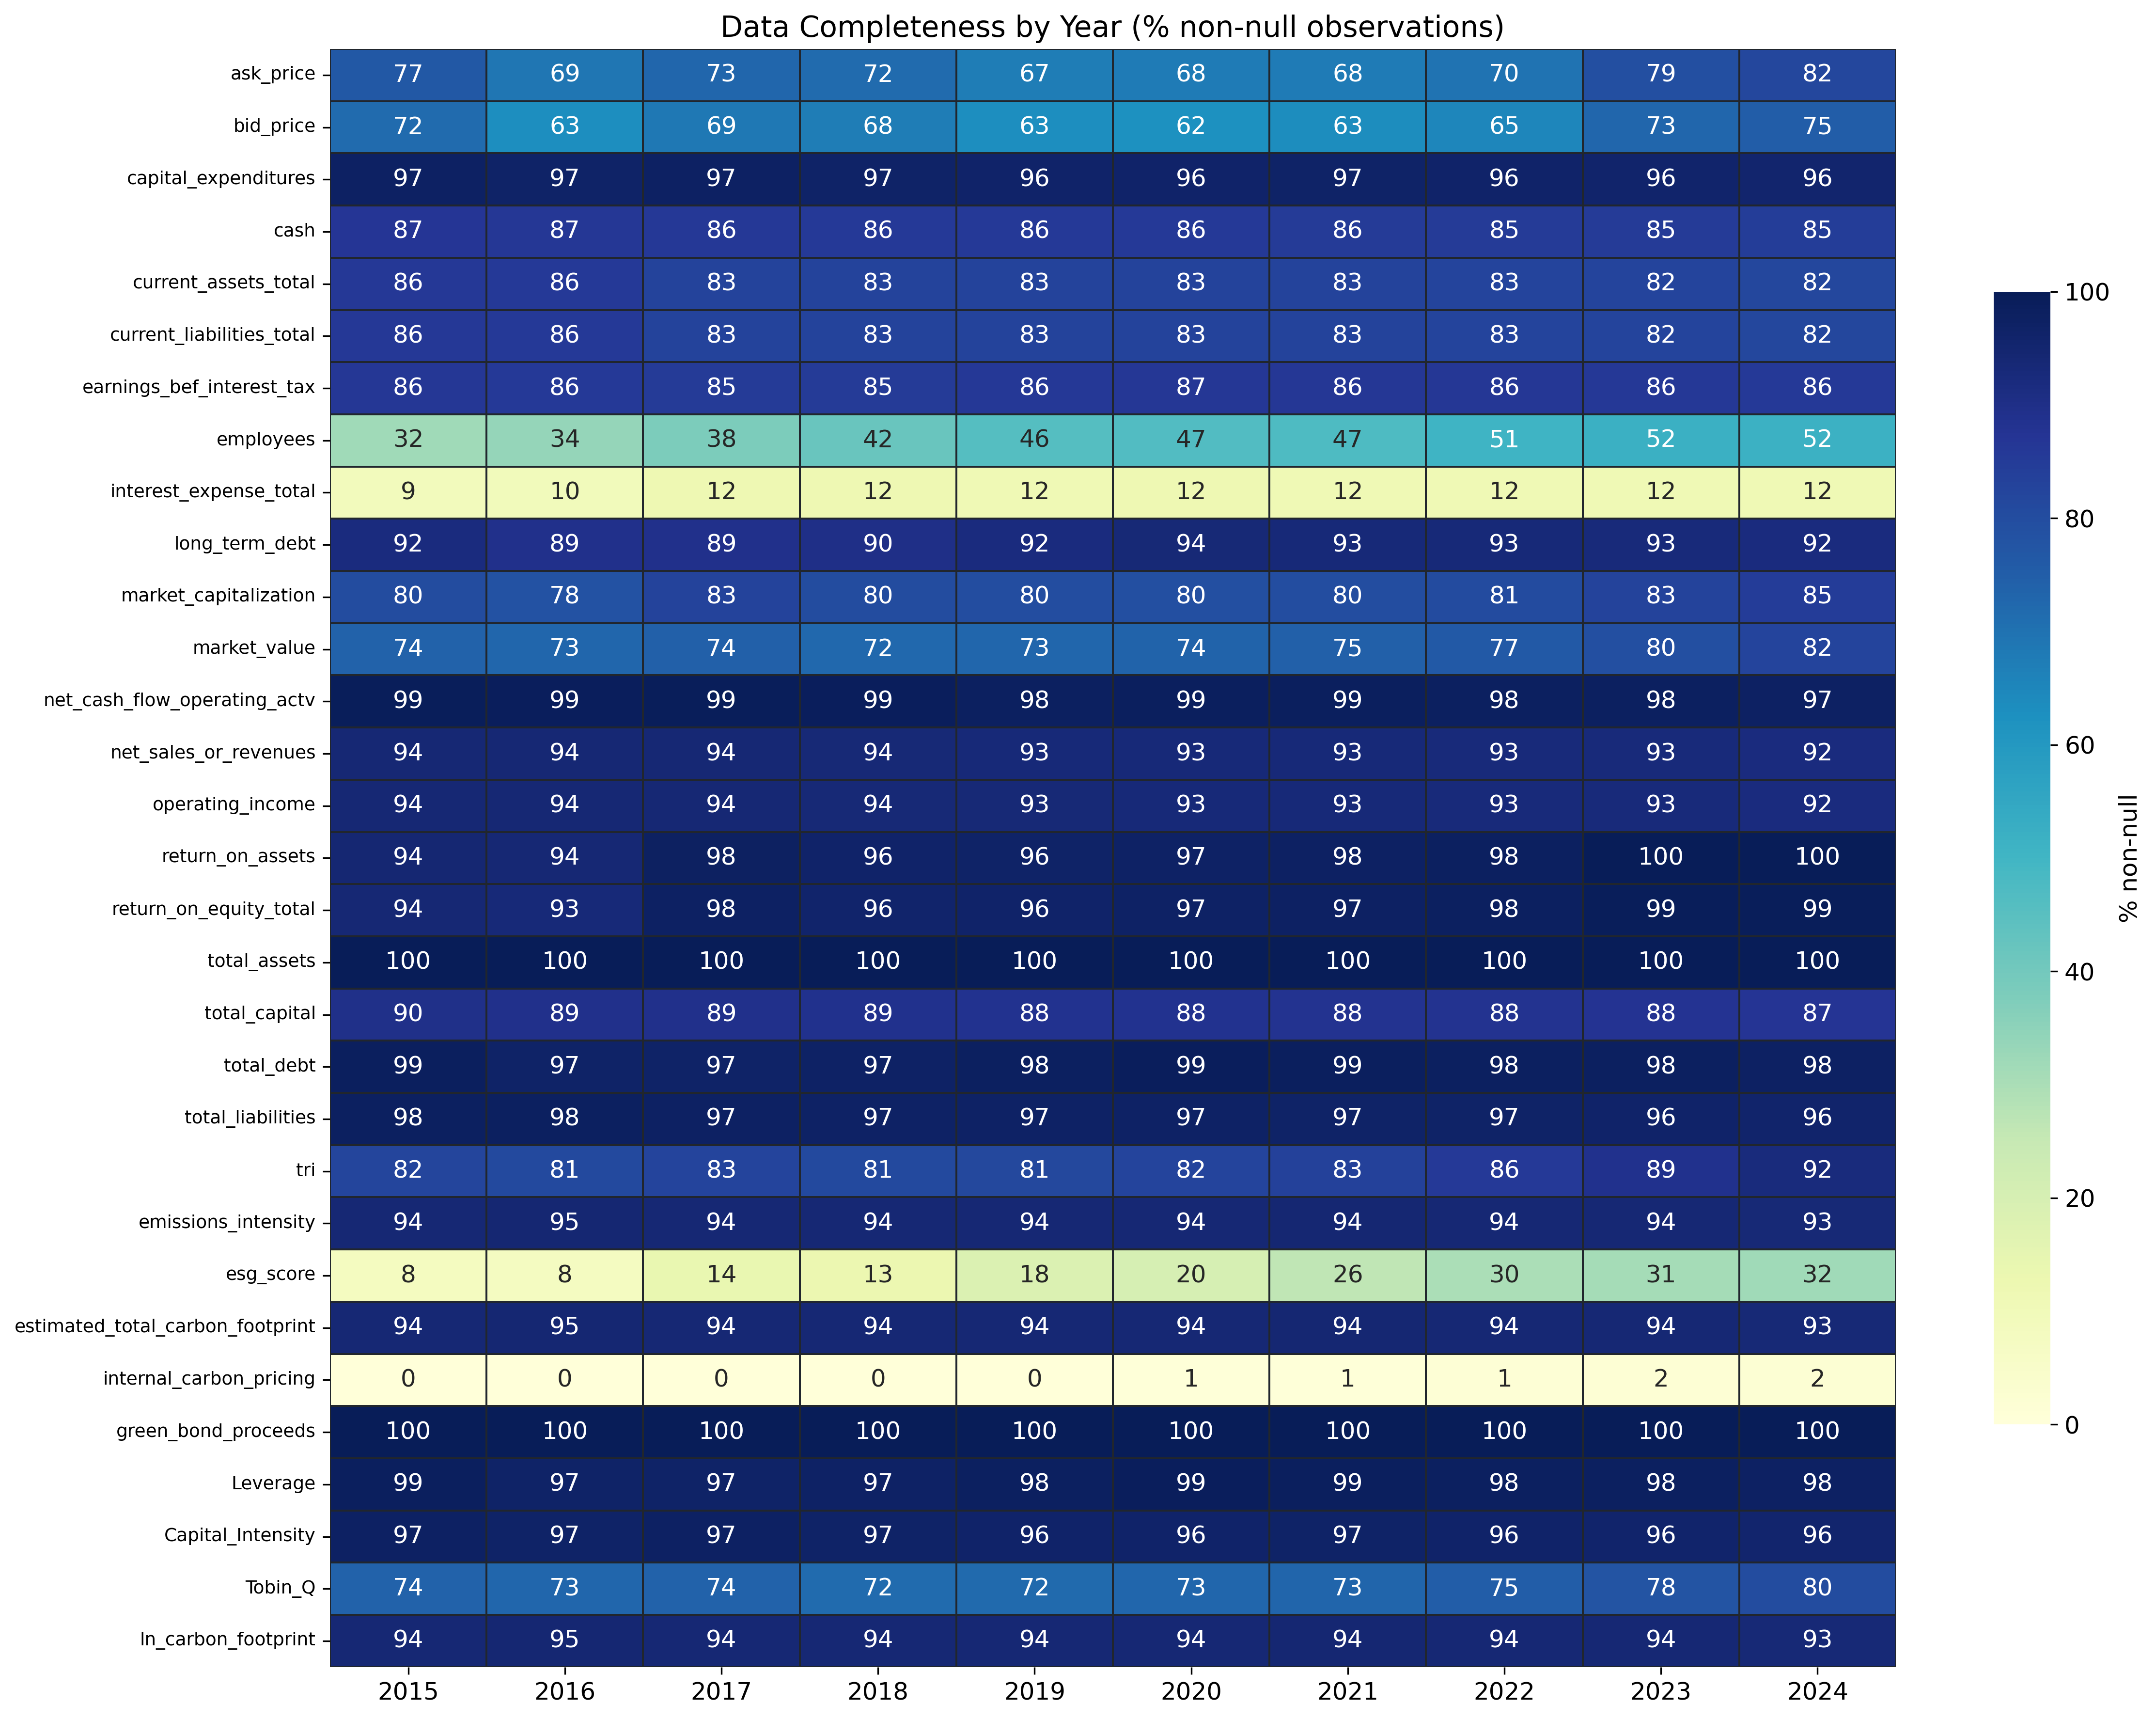
\includegraphics[width=0.75\textwidth]{../images/data_completeness.png}
               \caption{Coverage of numeric variables by year.}
            \end{figure}
        \end{column}
        \begin{column}{0.35\textwidth}
            \textbf{Key Insights:}
            \small
            \begin{itemize}
                \item High completeness for core financial metrics (Assets, Debt, Revenue) across the panel period.
                \item Significant gaps in specific ESG disclosures (e.g., ESG Score, Internal Carbon Pricing), particularly in earlier years.
                \item Highlights the challenge of sparse environmental data in regional analyses.
            \end{itemize}
        \end{column}
    \end{columns}
\end{frame}

% Section 2: Exploratory Data Analysis
\section{Exploratory Data Analysis}

% Slide 5: Trend Analysis
\begin{frame}{Trend Analysis: ASEAN-Level Averages}
    \begin{columns}
        \begin{column}{0.65\textwidth}
            \begin{figure}
               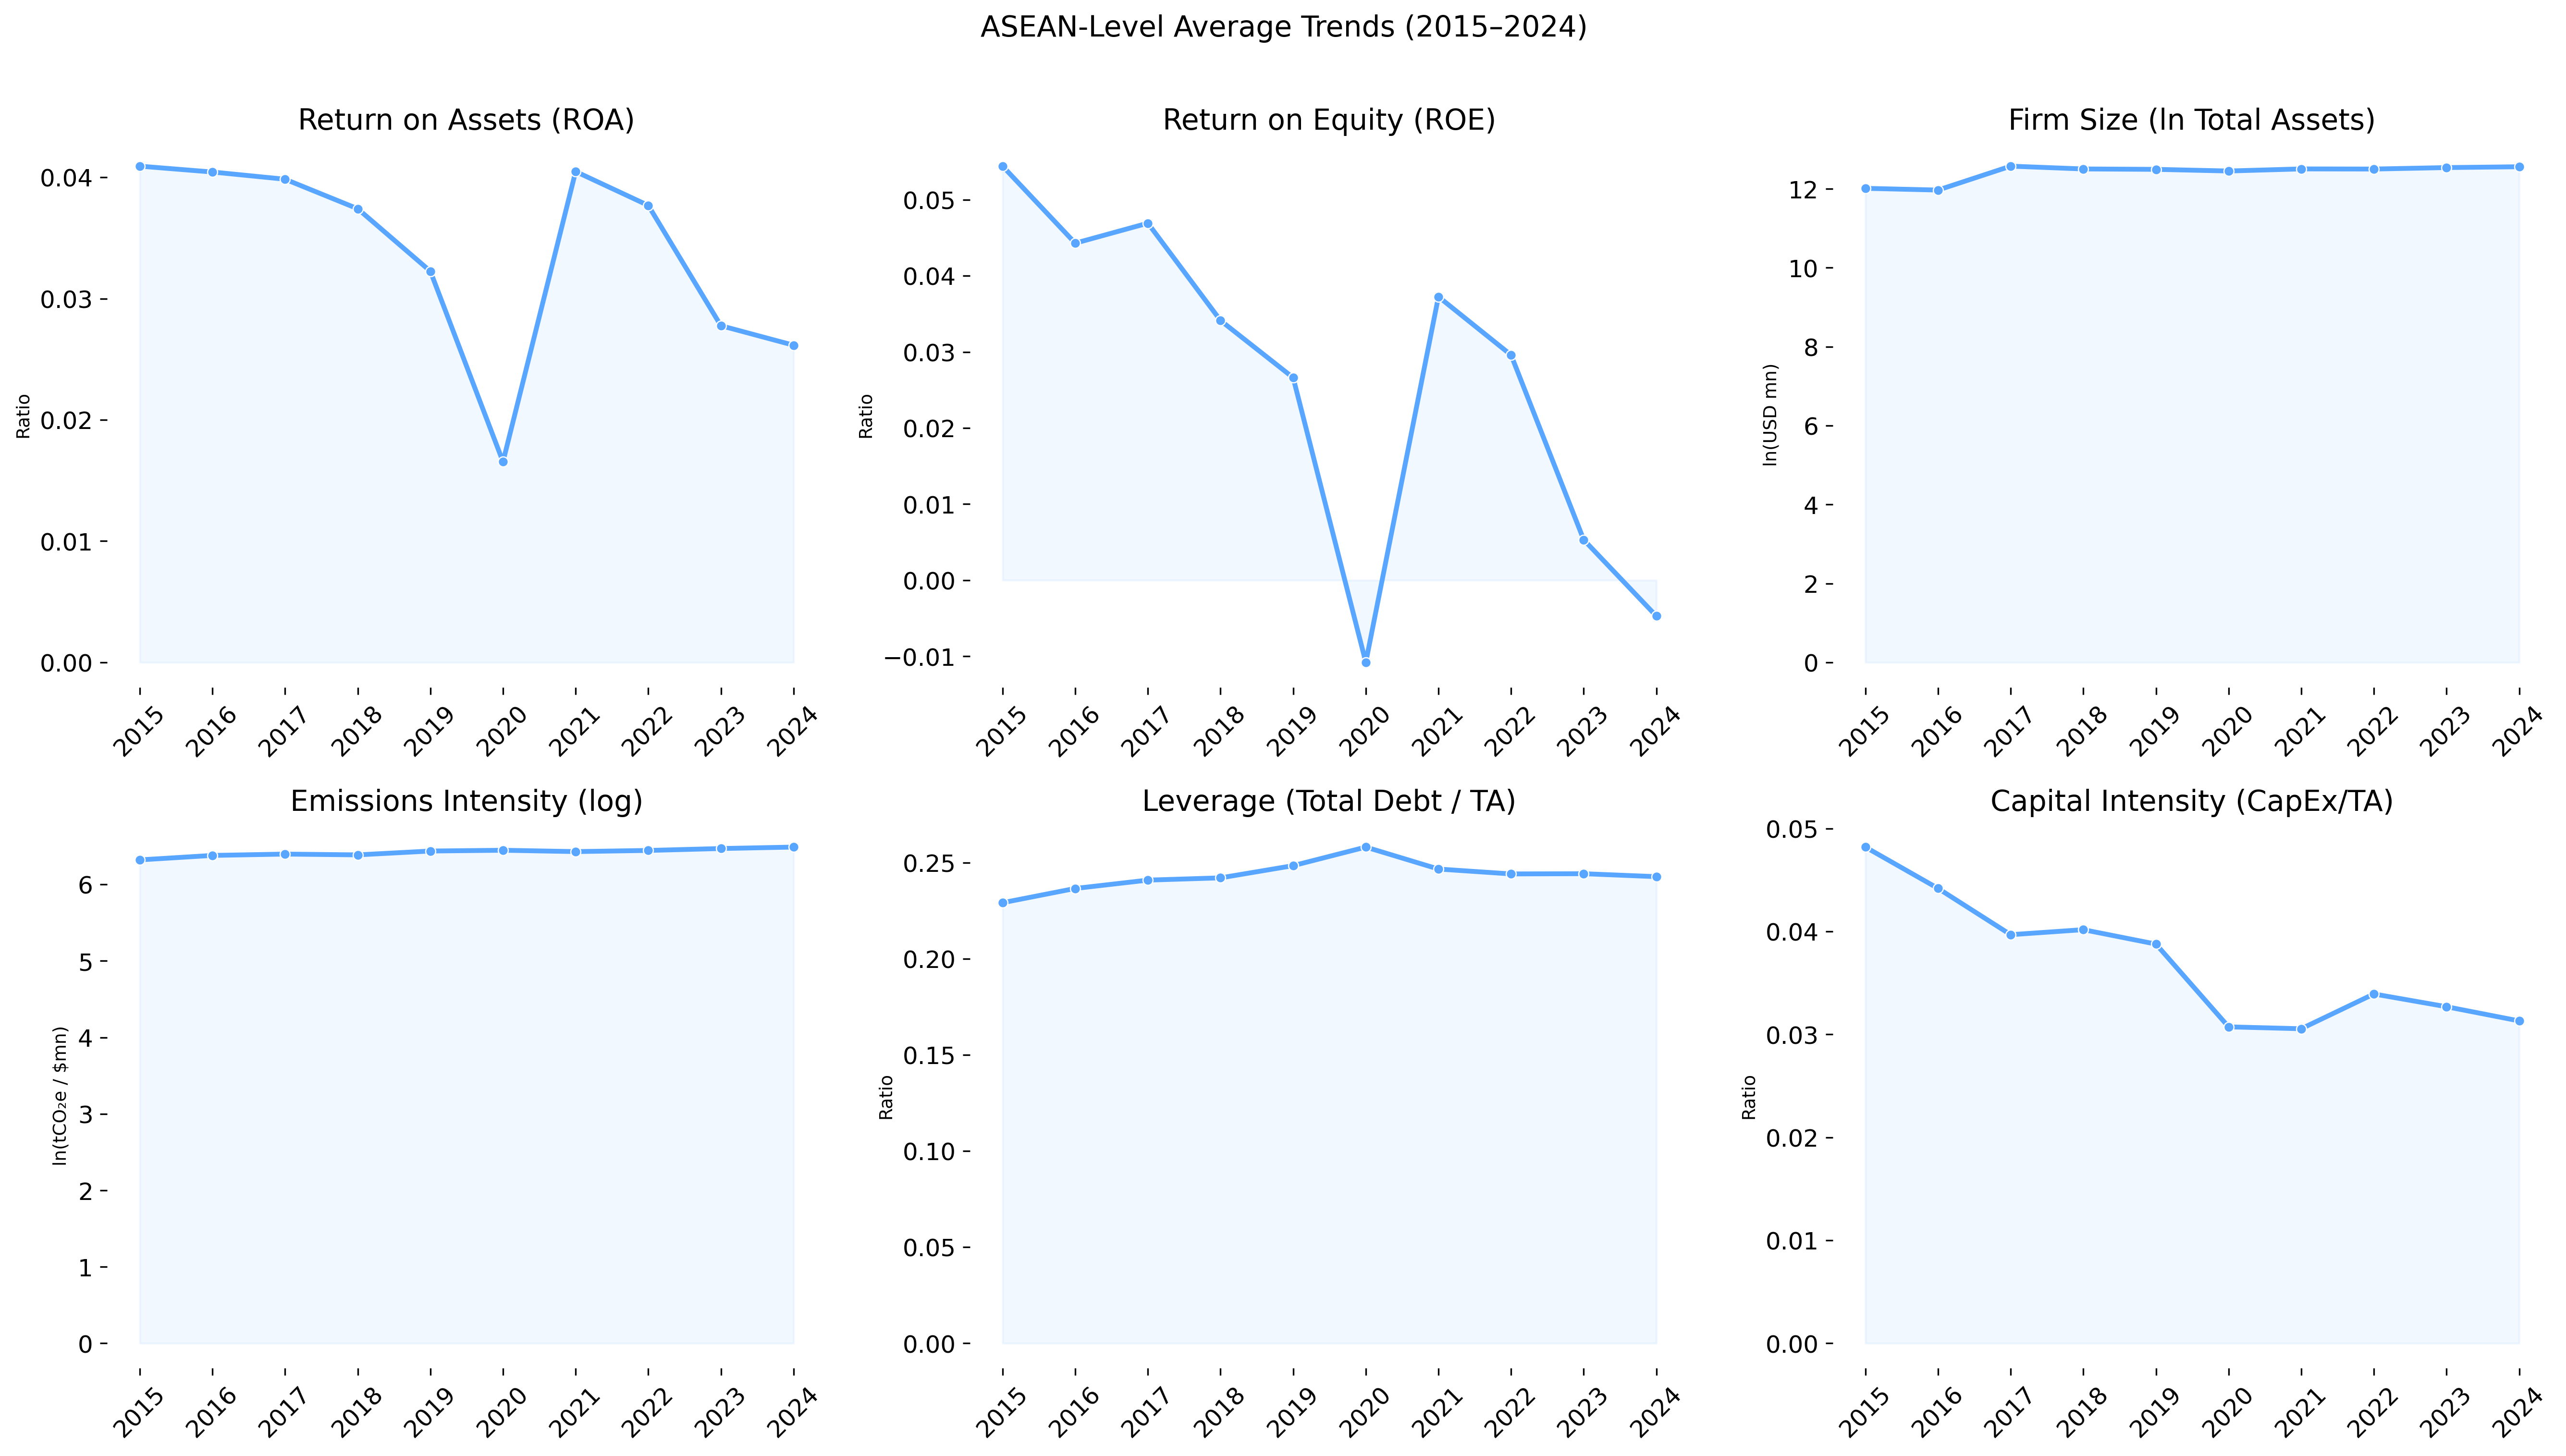
\includegraphics[width=\textwidth]{../images/trend_analysis.png}
               \caption{Average trajectory of core variables across the full panel.}
            \end{figure}
        \end{column}
        \begin{column}{0.35\textwidth}
            \textbf{Key Insights:}
            \begin{itemize}
                \item \textbf{Pandemic Impact:} Sharp dips in profitability (ROA and ROE) around 2020. ROA recovers strongly, but ROE exhibits a secondary decline in 2023--2024, suggesting persistent structural challenges.
                \item \textbf{Capital \& Leverage:} Capital intensity shows a gradually declining trend, while leverage and firm size remain highly stable over the decade.
                \item \textbf{Emissions:} Average emissions intensity remains relatively flat, indicating a slow overall transition at the macro level.
            \end{itemize}
        \end{column}
    \end{columns}
\end{frame}

% Slide 6: Sector & Country Financial Profiles
\begin{frame}{Country-Level Financial Profiles}
    \begin{columns}
        \begin{column}{0.6\textwidth}
            \begin{figure}
               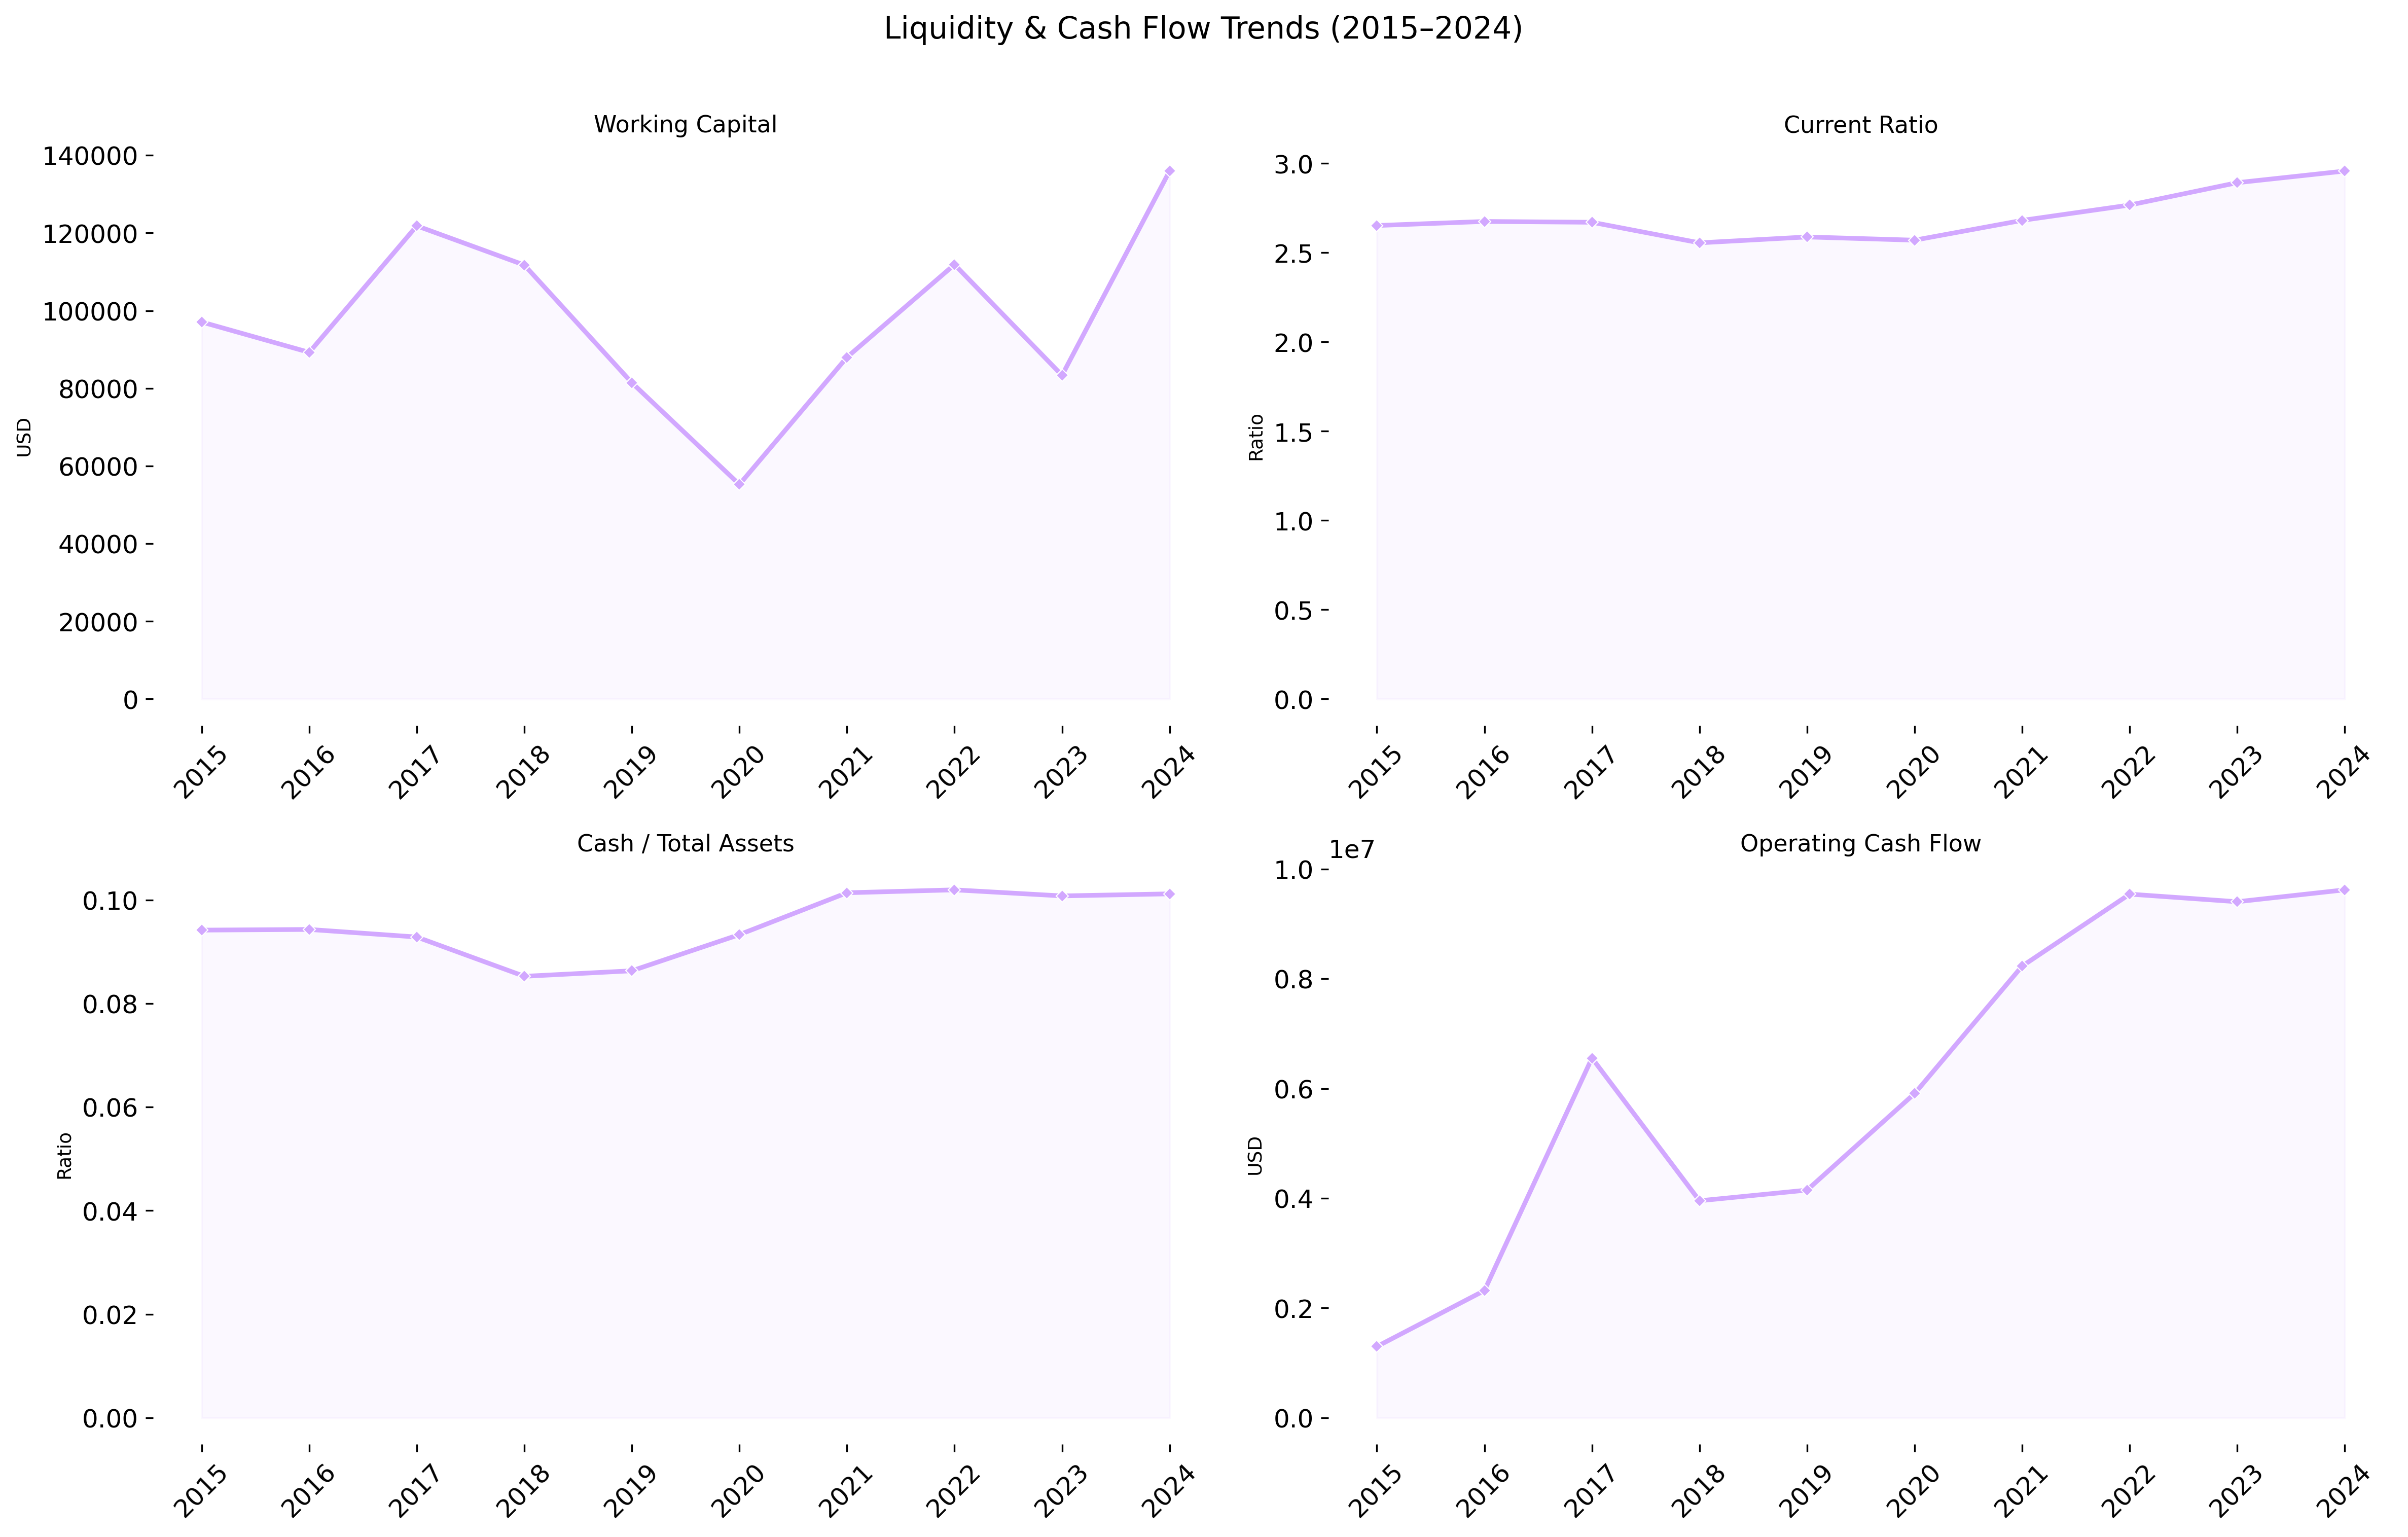
\includegraphics[width=\textwidth]{../images/sector_analysis.png}
               \caption{Financial Health by Country (2015--2024).}
            \end{figure}
        \end{column}
        \begin{column}{0.4\textwidth}
            \textbf{Key Insights:}
            \begin{itemize}
                \item \textbf{Scale Disparity:} Singapore-listed firms dominate in Total Assets, Revenue, and Debt, often 3--5$\times$ larger than peers.
                \item \textbf{COVID Impact:} Operating Income across all countries shows a visible dip at 2020, mirroring the ROA/ROE trends.
                \item \textbf{Implication:} The wide cross-country scale variation motivates the Firm Size $\times$ Green Bond interaction term and entity fixed effects.
            \end{itemize}
        \end{column}
    \end{columns}
\end{frame}

% Slide 7: Distribution & Outliers
\begin{frame}{Distribution \& Outlier Analysis}
    \begin{figure}
       \centering
       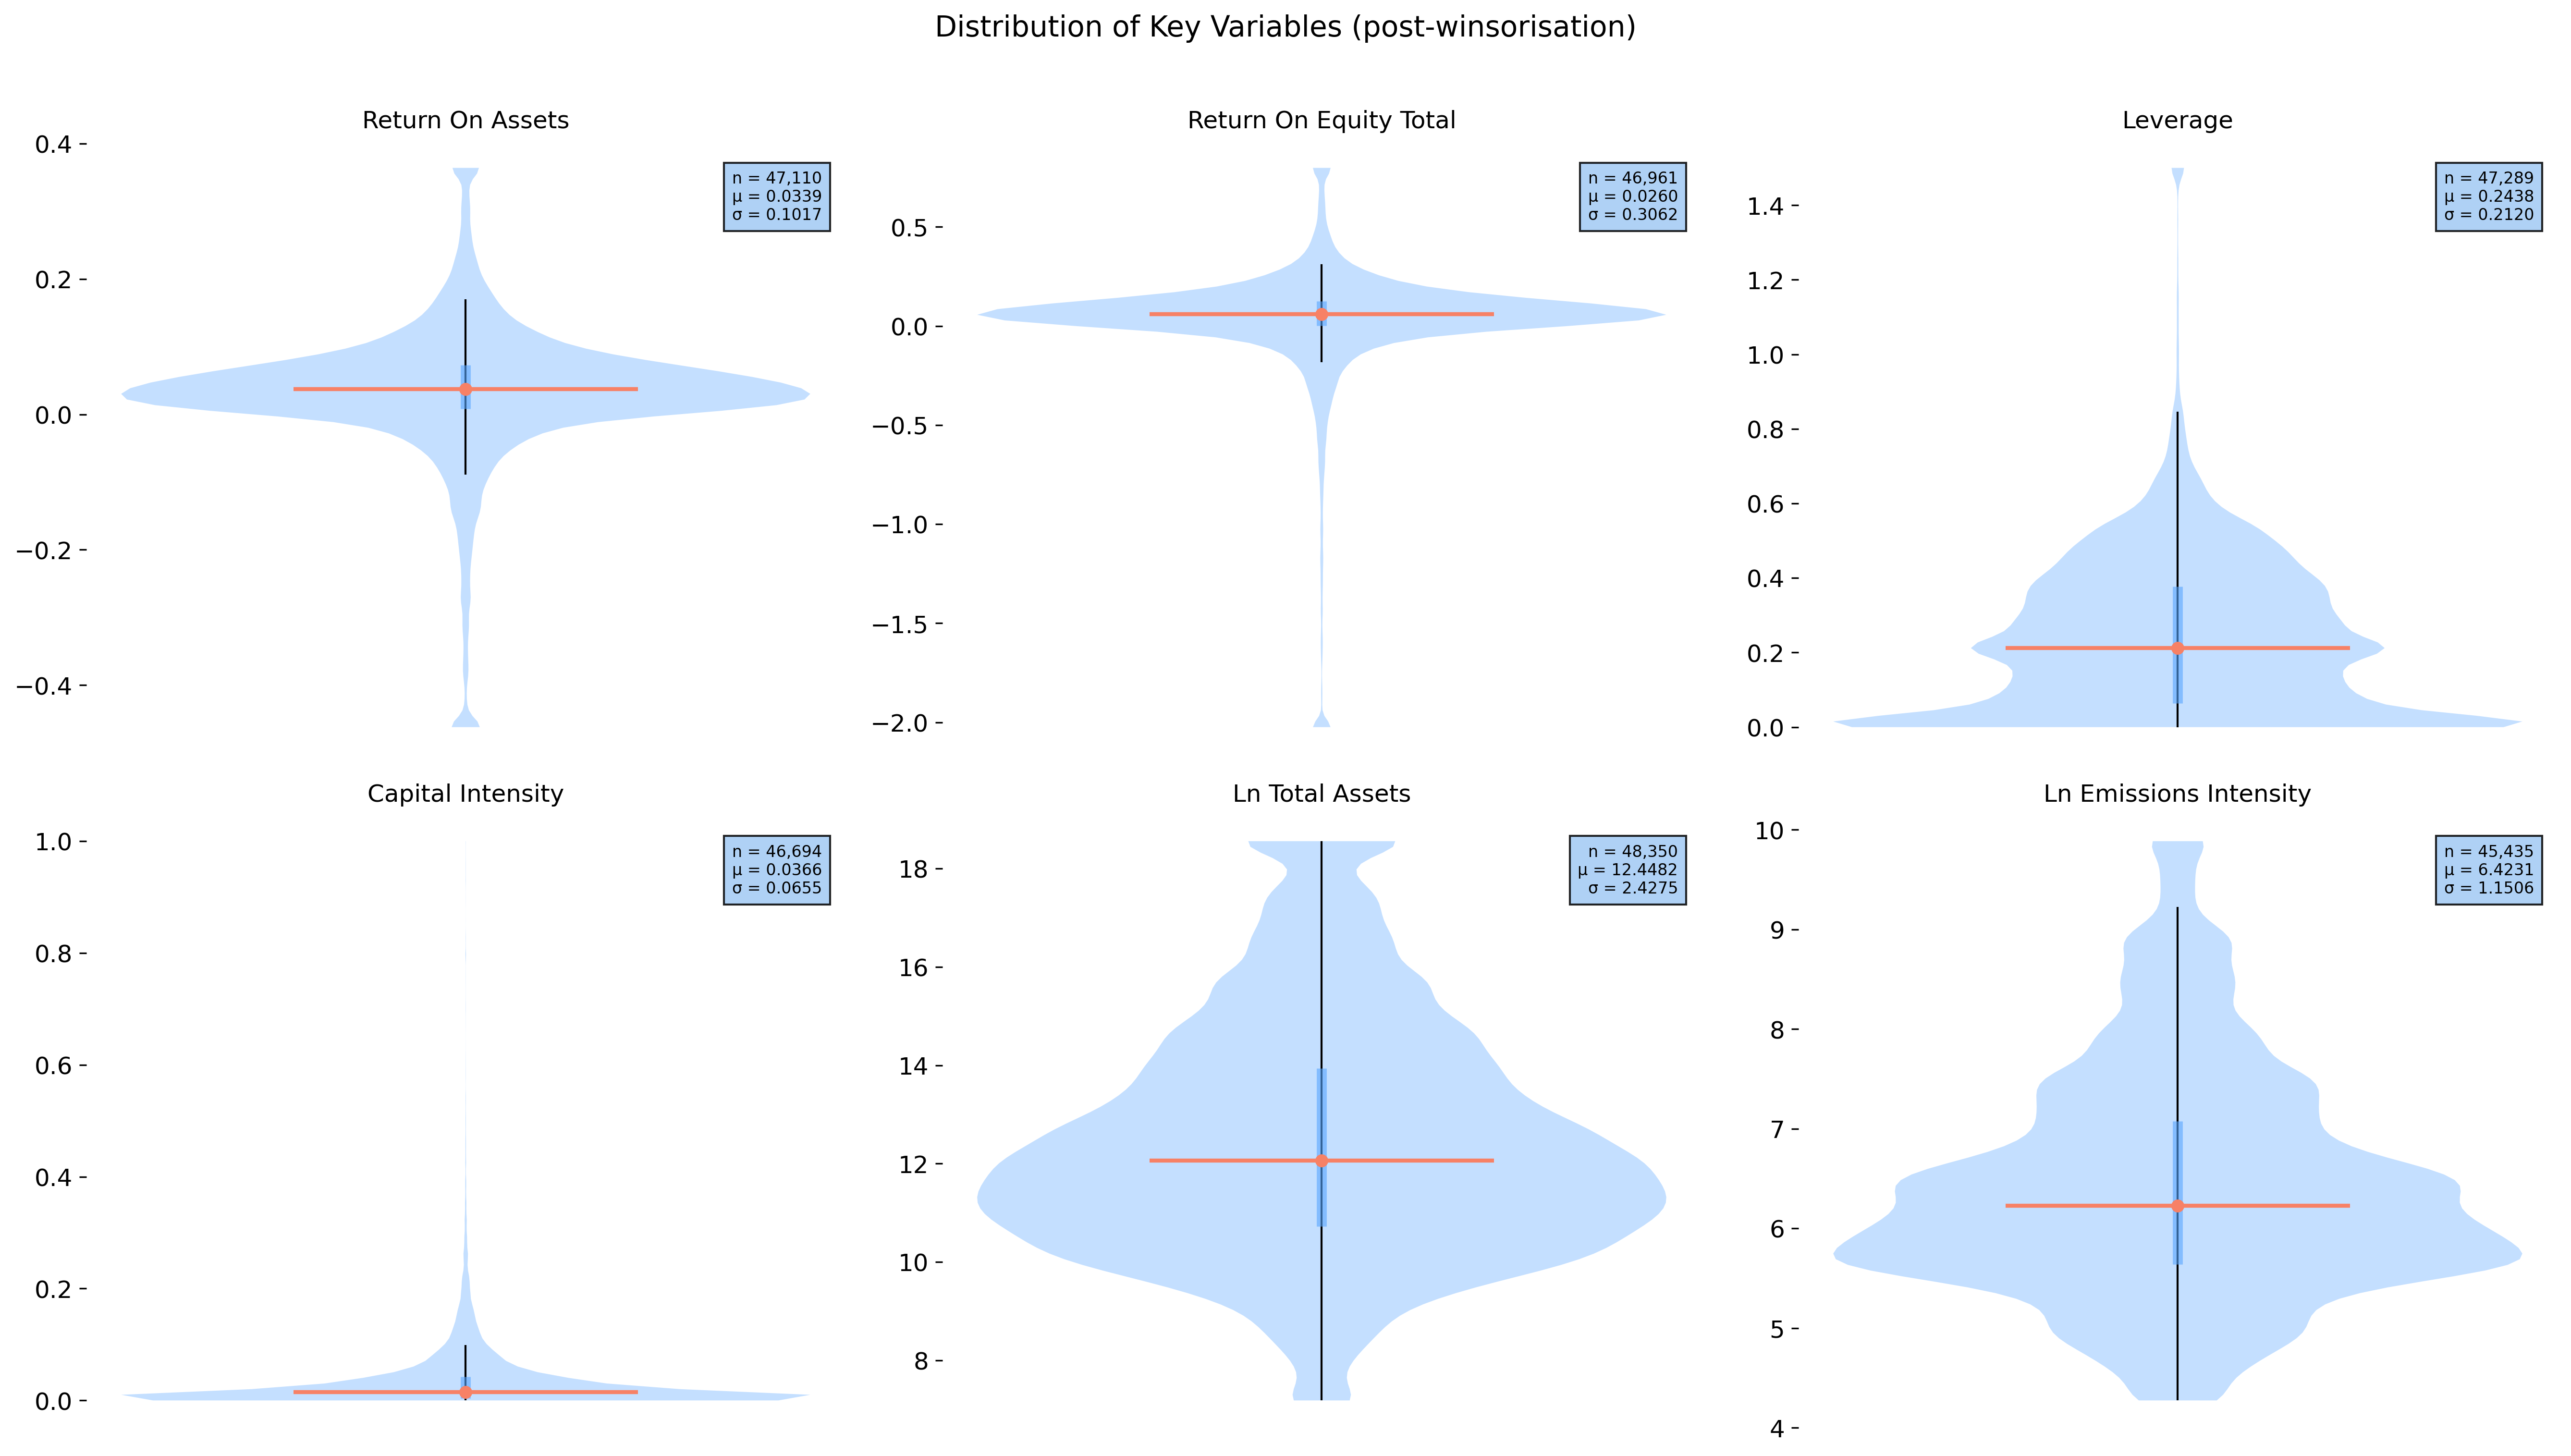
\includegraphics[width=0.38\textwidth]{../images/violin_plots.png} \hfill
       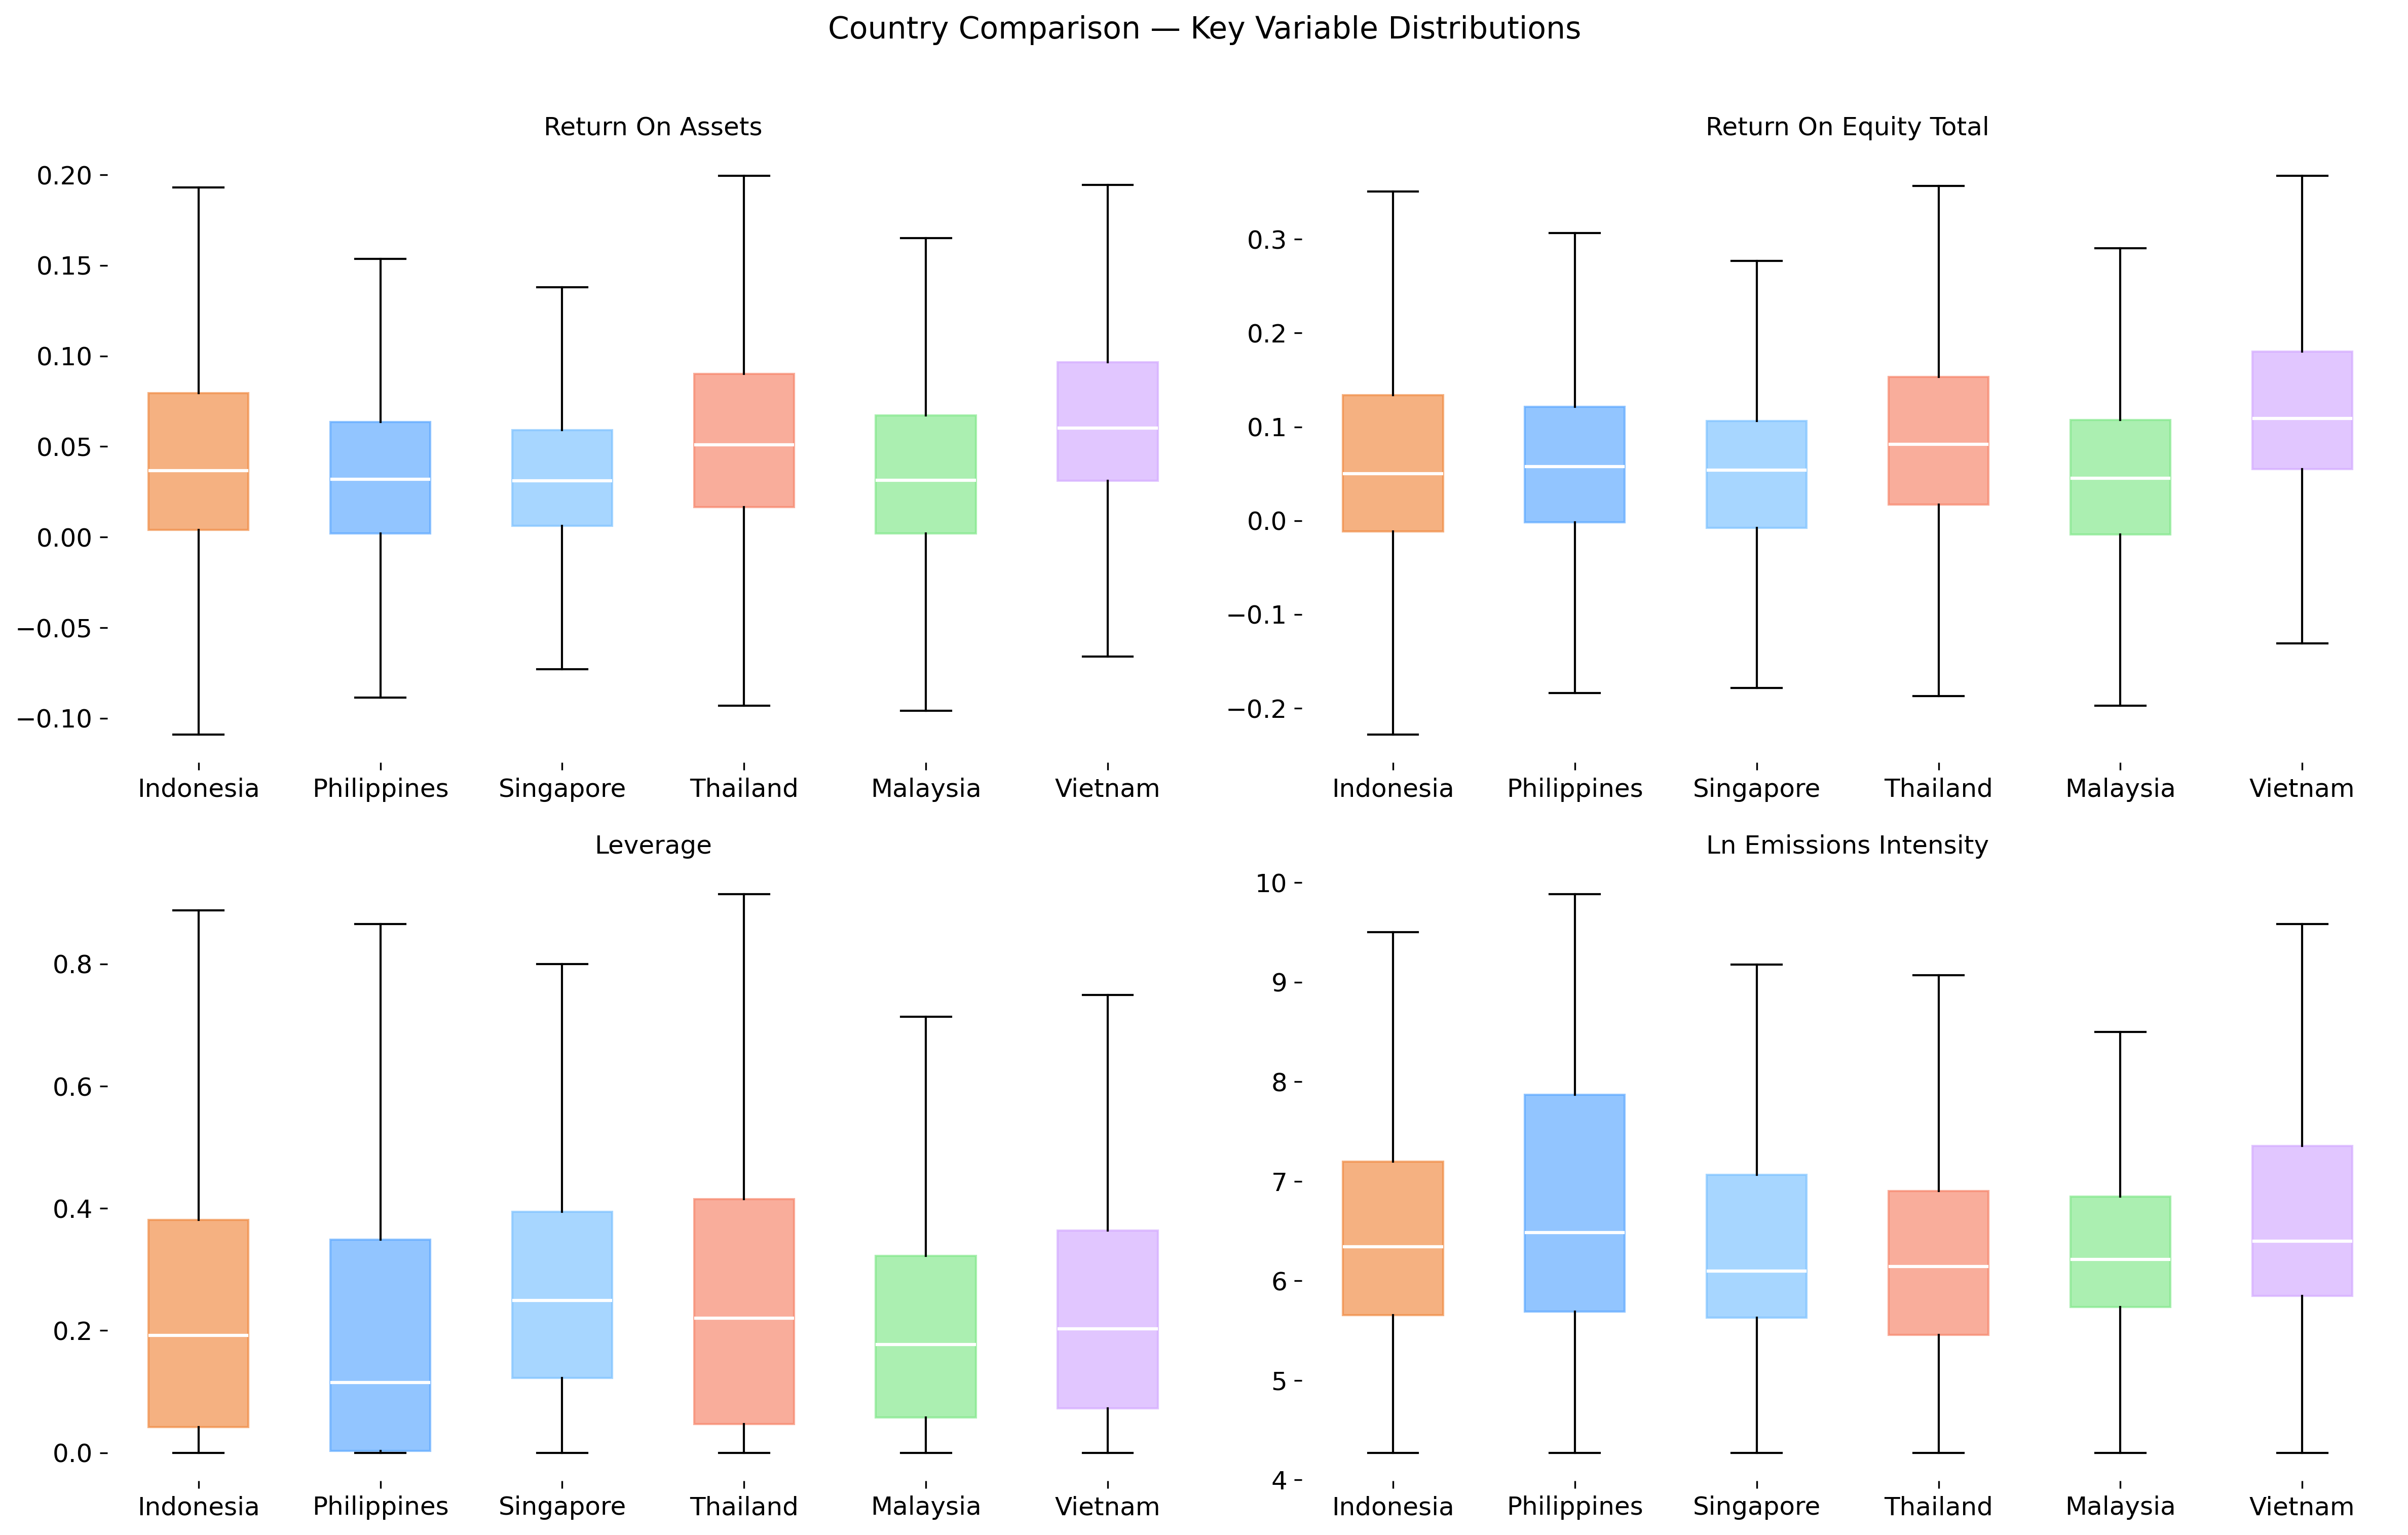
\includegraphics[width=0.38\textwidth]{../images/box_plots.png}
       \caption{Violin plots and Box plots for key continuous variables.}
    \end{figure}
    \vspace{-0.3cm}
    \small
    \begin{itemize}
        \item \textbf{Financials:} ROA and ROE exhibit tight, slightly positive-centered distributions; ROE shows notably heavy tails.
        \item \textbf{Emissions:} Log-transformed emissions intensity shows a smoother, more normal distribution post-winsorization.
        \item \textbf{Implication:} Residual non-normality persists, justifying robust/clustered standard errors.
    \end{itemize}
\end{frame}

% Section 3: Deep Dive into Green Bonds
\section{Green Bond Deep Dive \& Intervening Dynamics}

% Slide 8: Green Bond Issuance Overview
\begin{frame}{Green Bond Deep Dive: Issuance Patterns}
    \begin{columns}
        \begin{column}{0.6\textwidth}
            \begin{figure}
               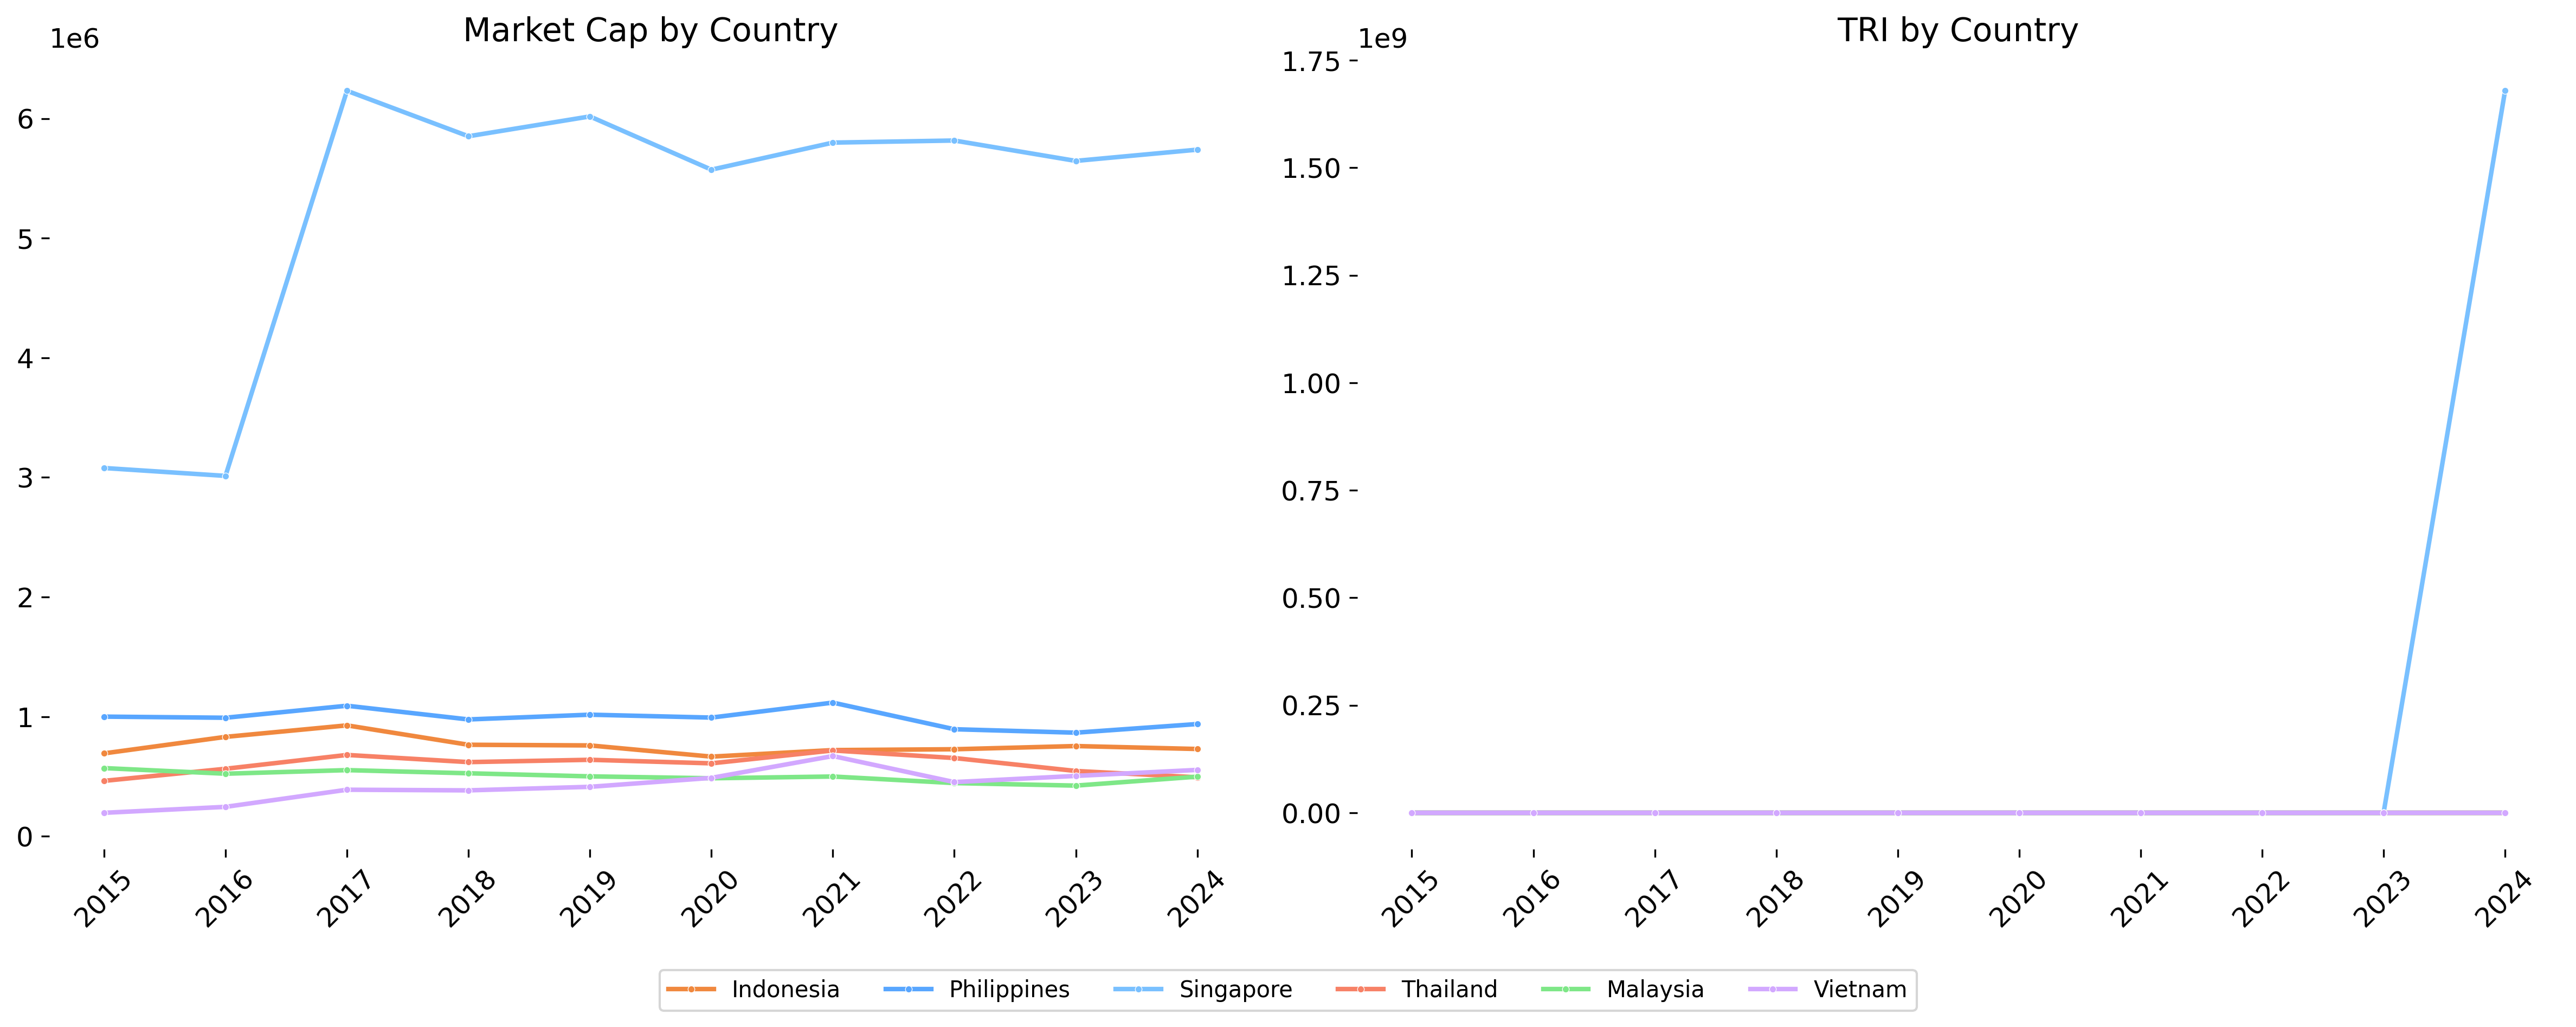
\includegraphics[width=\textwidth]{../images/green_bond_patterns.png}
               \caption{Green bond issuance events and proceeds by year.}
            \end{figure}
        \end{column}
        \begin{column}{0.4\textwidth}
            \textbf{Key Insights:}
            \begin{itemize}
                \item \textbf{Peak Activity:} 2020 saw the highest issuance volume (7 events) and proceeds, driven by Indonesia and Singapore.
                \item \textbf{Regional Breadth:} Thailand, Indonesia, Singapore, Philippines, and Vietnam all contribute, with Malaysia entering in 2023--2024.
                \item \textbf{Staggered Adoption:} The variation in issuance timing across countries provides a natural foundation for staggered Difference-in-Differences estimation.
            \end{itemize}
        \end{column}
    \end{columns}
\end{frame}

% Slide 8: DID Pre-Check: Parallel Trends
\begin{frame}{DID Pre-Check: Parallel Trends Assumption}
    \begin{columns}
        \begin{column}{0.6\textwidth}
            \begin{figure}
               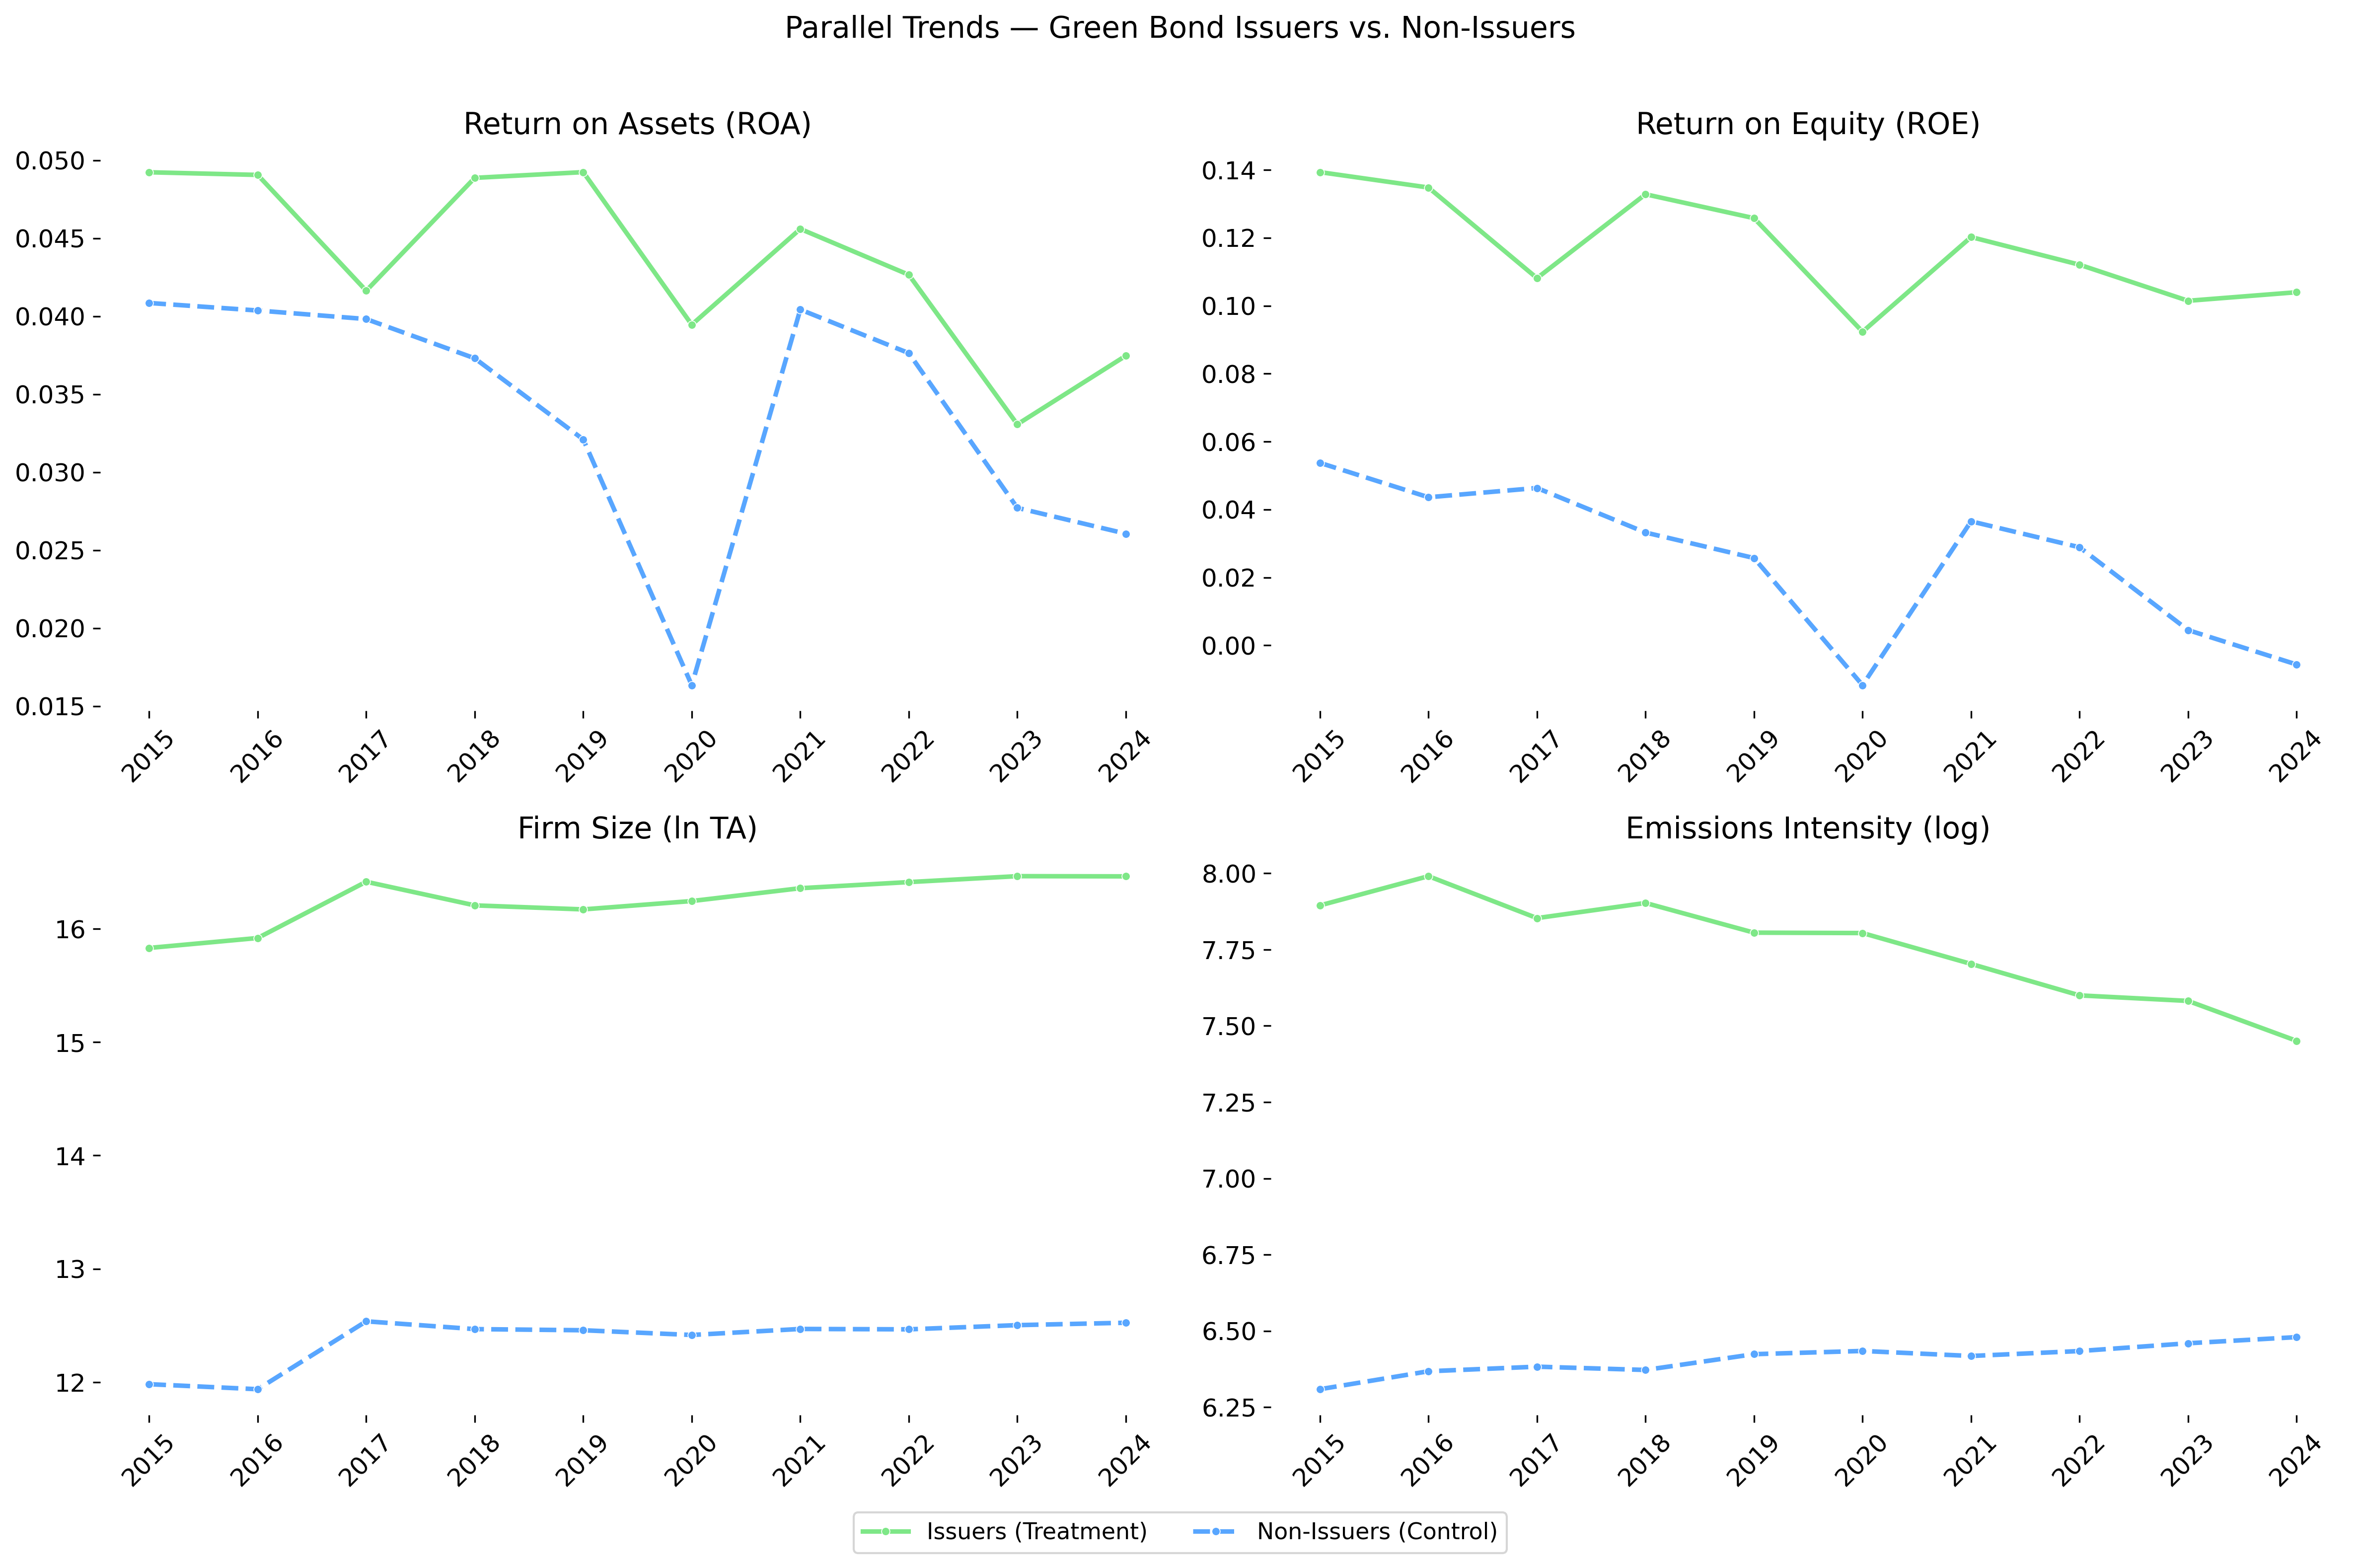
\includegraphics[width=\textwidth]{../images/parallel_trends.png}
               \caption{Pre-treatment trends: Issuers vs. Non-Issuers.}
            \end{figure}
        \end{column}
        \begin{column}{0.4\textwidth}
            \textbf{Key Insights:}
            \begin{itemize}
                \item \textbf{Financials (ROA/ROE):} Both groups follow approximately similar pre-issuance trajectories, though issuers exhibit higher volatility.
                \item \textbf{Size \& Emissions:} Issuers are larger with distinct emissions levels; post-treatment, issuers' emissions decline while non-issuers' slightly rise---a potential treatment effect signal.
                \item \textbf{Assessment:} Visual inspection suggests pre-treatment trends are approximately parallel; formal event-study leads are recommended to confirm.
            \end{itemize}
        \end{column}
    \end{columns}
\end{frame}

% Slide 9: Feature Correlation \& Market Performance
\begin{frame}{Feature Correlation \& Market Performance}
    \begin{columns}
        \begin{column}{0.55\textwidth}
            \begin{figure}
               \centering
               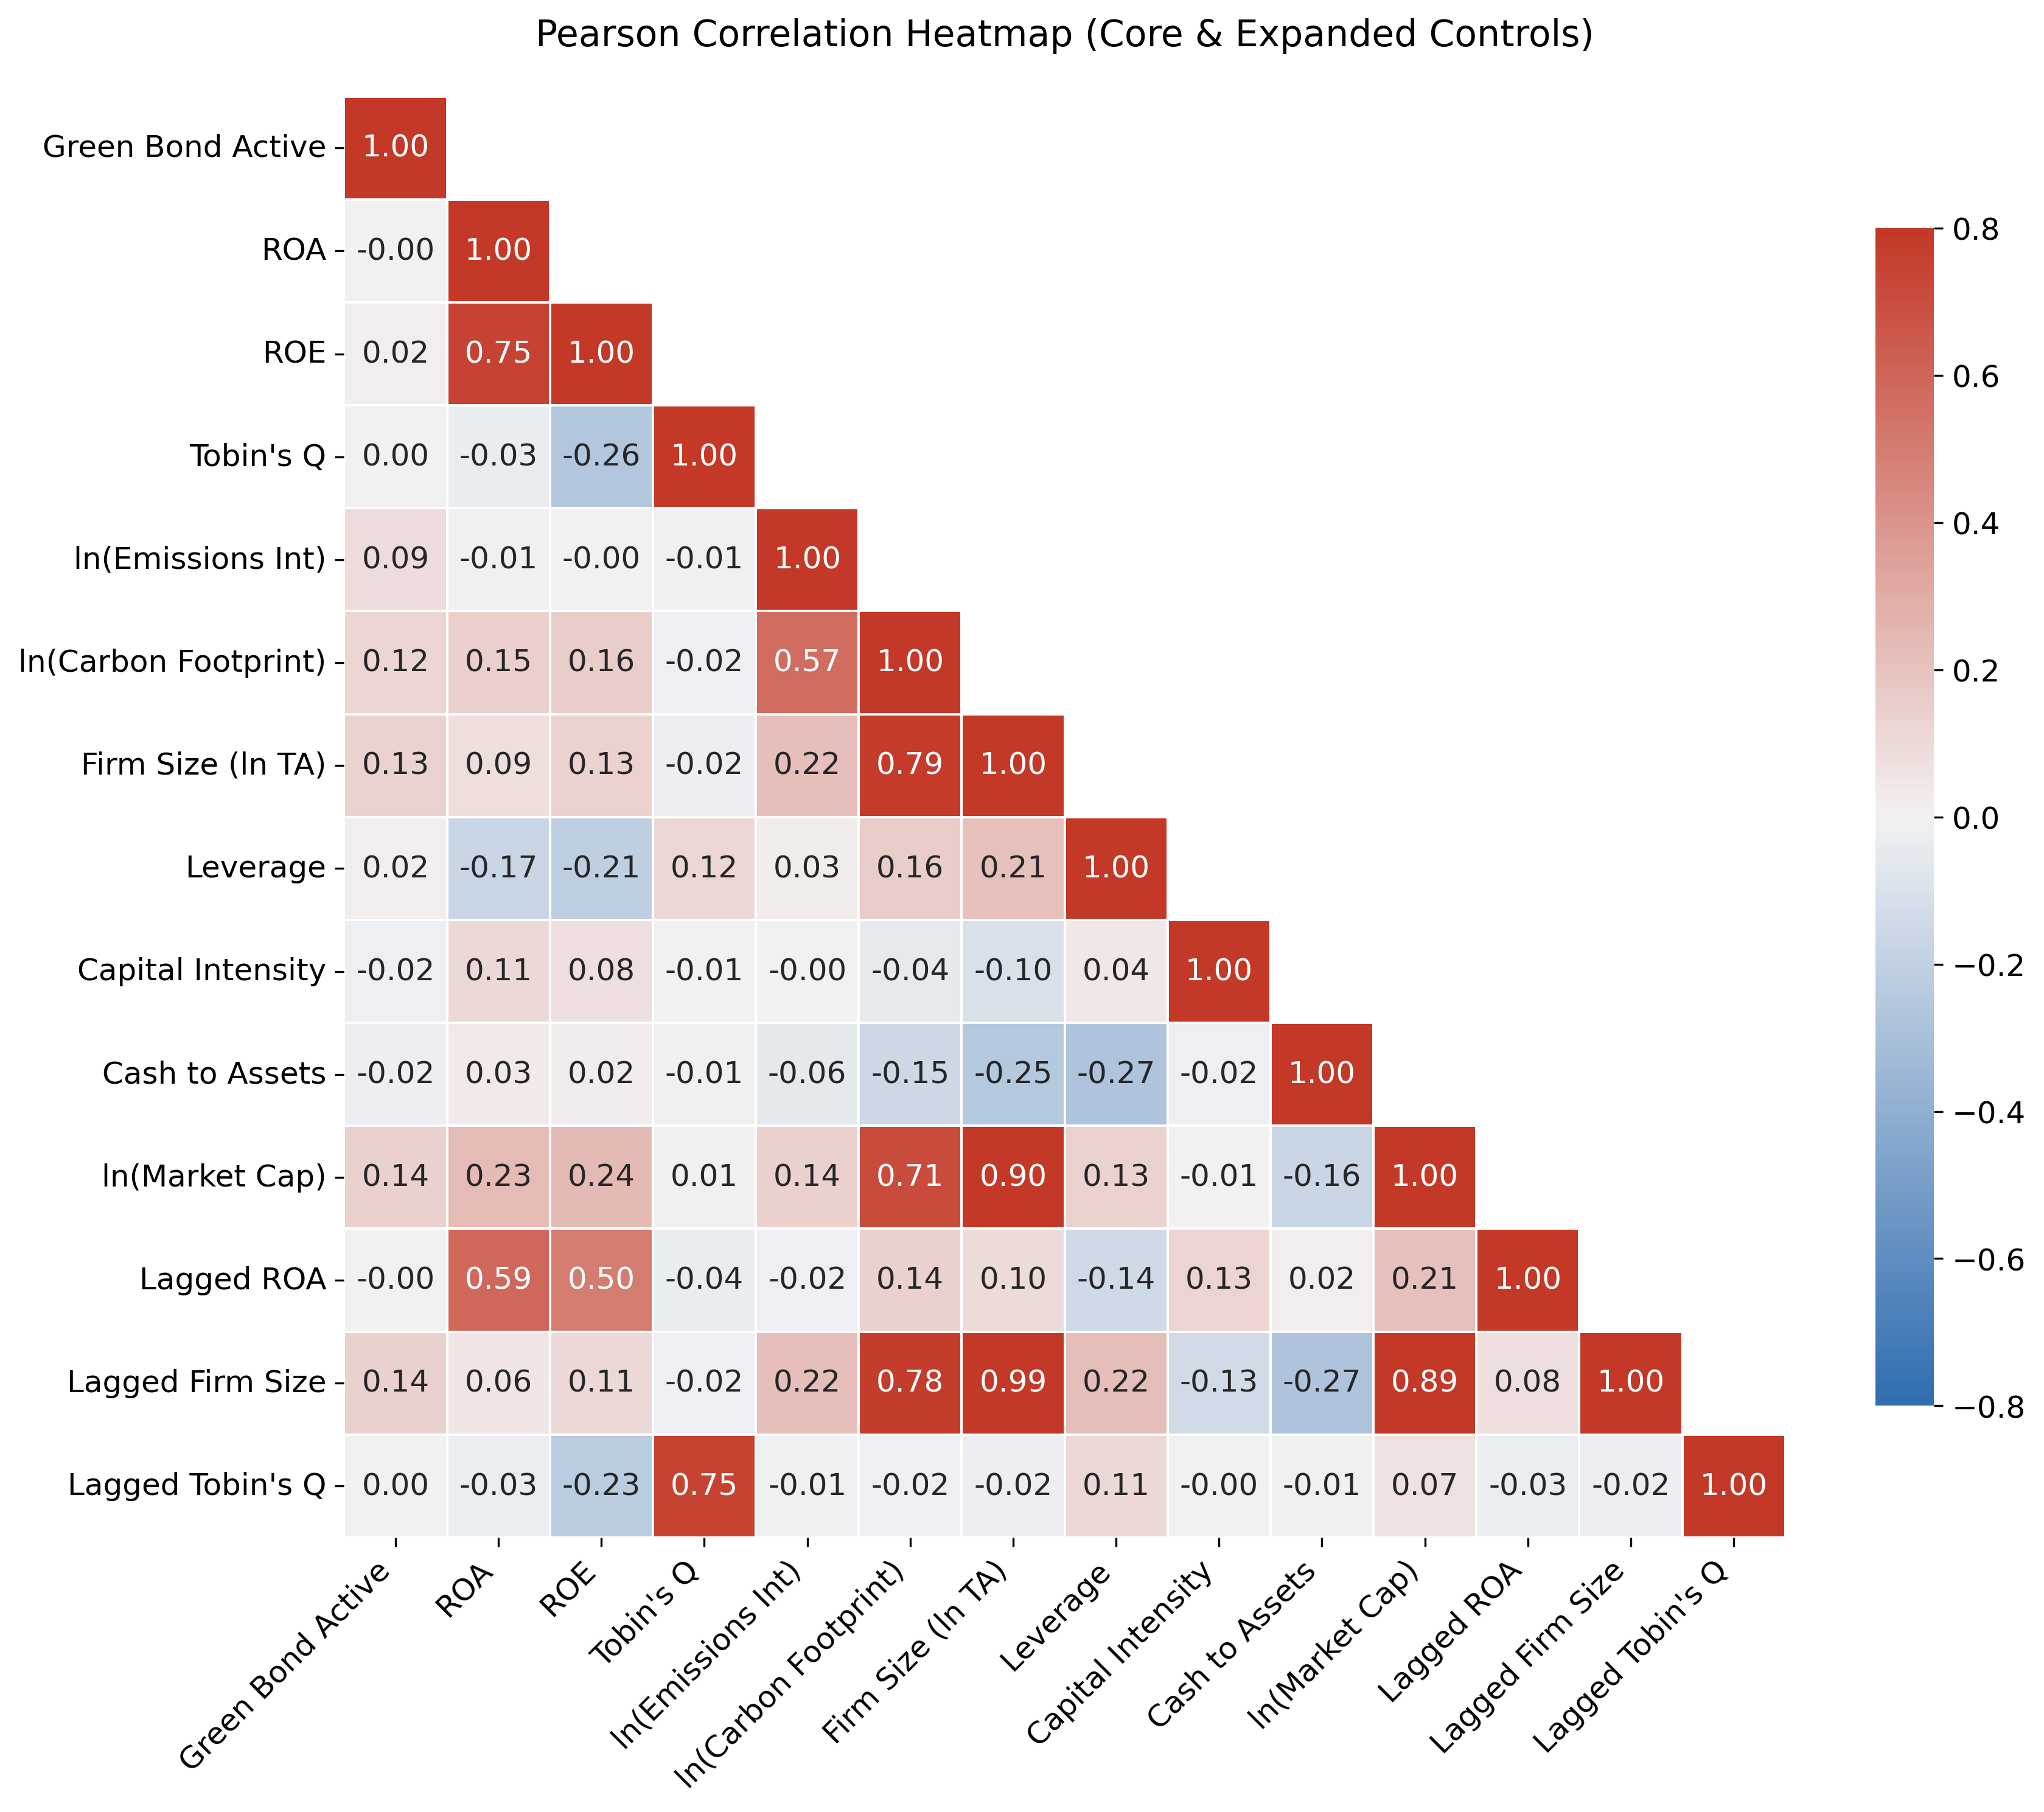
\includegraphics[width=0.85\textwidth]{../images/correlation_heatmap.png}
               \caption{Pearson Correlations (Core Subset).}
            \end{figure}
        \end{column}
        \begin{column}{0.45\textwidth}
            \textbf{Key Insights:}
            \begin{itemize}
                \item \textbf{Multicollinearity:} Firm Size and Market Cap are highly correlated ($r=0.87$); lagged variables show near-unity correlation ($r=0.99$) with their contemporaneous values---these pairs should not enter models simultaneously.
                \item \textbf{Relationships:} ROA--ROE correlation ($r=0.74$) supports using them as separate dependent variables rather than joint regressors. Other cross-variable correlations are moderate.
                \item \textbf{Modeling Needs:} VIF diagnostics and careful variable selection are warranted alongside interaction terms and fixed-effects.
            \end{itemize}
        \end{column}
    \end{columns}
\end{frame}

% Section 4: Advanced Characteristics & Heterogeneity
\section{Key Heterogeneous Effects}

% Slide 10: Interaction Effects - Firm Size & Leverage
\begin{frame}{Interaction Effects: Size \& Leverage}
    \begin{itemize}
        \item \textbf{Firm Size $\times$ Green Bond:}
        \begin{itemize}
            \item \textit{Rationale:} Large firms draw more market attention and benefit more from reputational boosts. 
            \item \textit{Impact:} Potential amplification of the environmental performance shock and efficiency of capital deployment.
        \end{itemize}
        \vspace{0.3cm}
        \item \textbf{Leverage $\times$ Green Bond:}
        \begin{itemize}
            \item \textit{Rationale:} Issuing an instrument adds debt layer; high preexisting debt increases financial distress risks.
            \item \textit{Impact:} Lower capacity to absorb new debt may counteract the so-called ``greenium.''
        \end{itemize}
    \end{itemize}
\end{frame}

% Slide 11: Interaction Effects - Cash & Sectors
\begin{frame}{Interaction Effects: Liquid Slack \& Sector Heterogeneity}
    \begin{itemize}
        \item \textbf{Cash-to-Assets $\times$ Green Bond:}
        \begin{itemize}
            \item \textit{Rationale:} Cash-constrained firms might realize massive positive NPV by having new access to green financing. Alternatively, cash-rich firms issuing green bonds might face ``greenwashing'' market skepticism.
        \end{itemize}
        \vspace{0.3cm}
        \item \textbf{Sector Dummies $\times$ Green Bond:}
        \begin{itemize}
            \item \textit{Rationale:} Materiality of environmental action differs globally (e.g. Utilities/Energy transitioning vs. IT/Financials operations).
            \item \textit{Impact:} Allows estimating whether performance impacts are entirely driven by heavy-emissions sectors transitioning properly.
        \end{itemize}
    \end{itemize}
\end{frame}

% Section 5: Conclusion
\section{Conclusion \& Next Steps}

% Slide 13: Visual Recap & Implications
\begin{frame}{Visual Recap \& Early Implications}
    \begin{itemize}
        \item \textbf{Robust Fundamentals:} Panel visualizations validate dataset integrity with expected financial distributions. Country-level profiles reveal substantial cross-market scale differences.
        \item \textbf{Methodological Soundness:} Approximate parallel pre-trends between Issuers and Non-Issuers support DID/PSM strategy; formal event-study tests are recommended.
        \item \textbf{Heterogeneous Channels:} Distribution and correlation analyses confirm that the impact of green bonds depends on firm-specific mechanics: \textbf{Size, Liquidity, Leverage, and Sector Materiality}.
    \end{itemize}
\end{frame}

\begin{frame}[c]
    \centering
    \Huge \textbf{Questions \& Discussion}
\end{frame}

% ============================================================
% APPENDIX
% ============================================================
\appendix
\section{Appendix}

% Appendix A: Country-Level Trends
\begin{frame}{Appendix A: Country-Level Trend Analysis}
    \begin{columns}
        \begin{column}{0.65\textwidth}
            \begin{figure}
               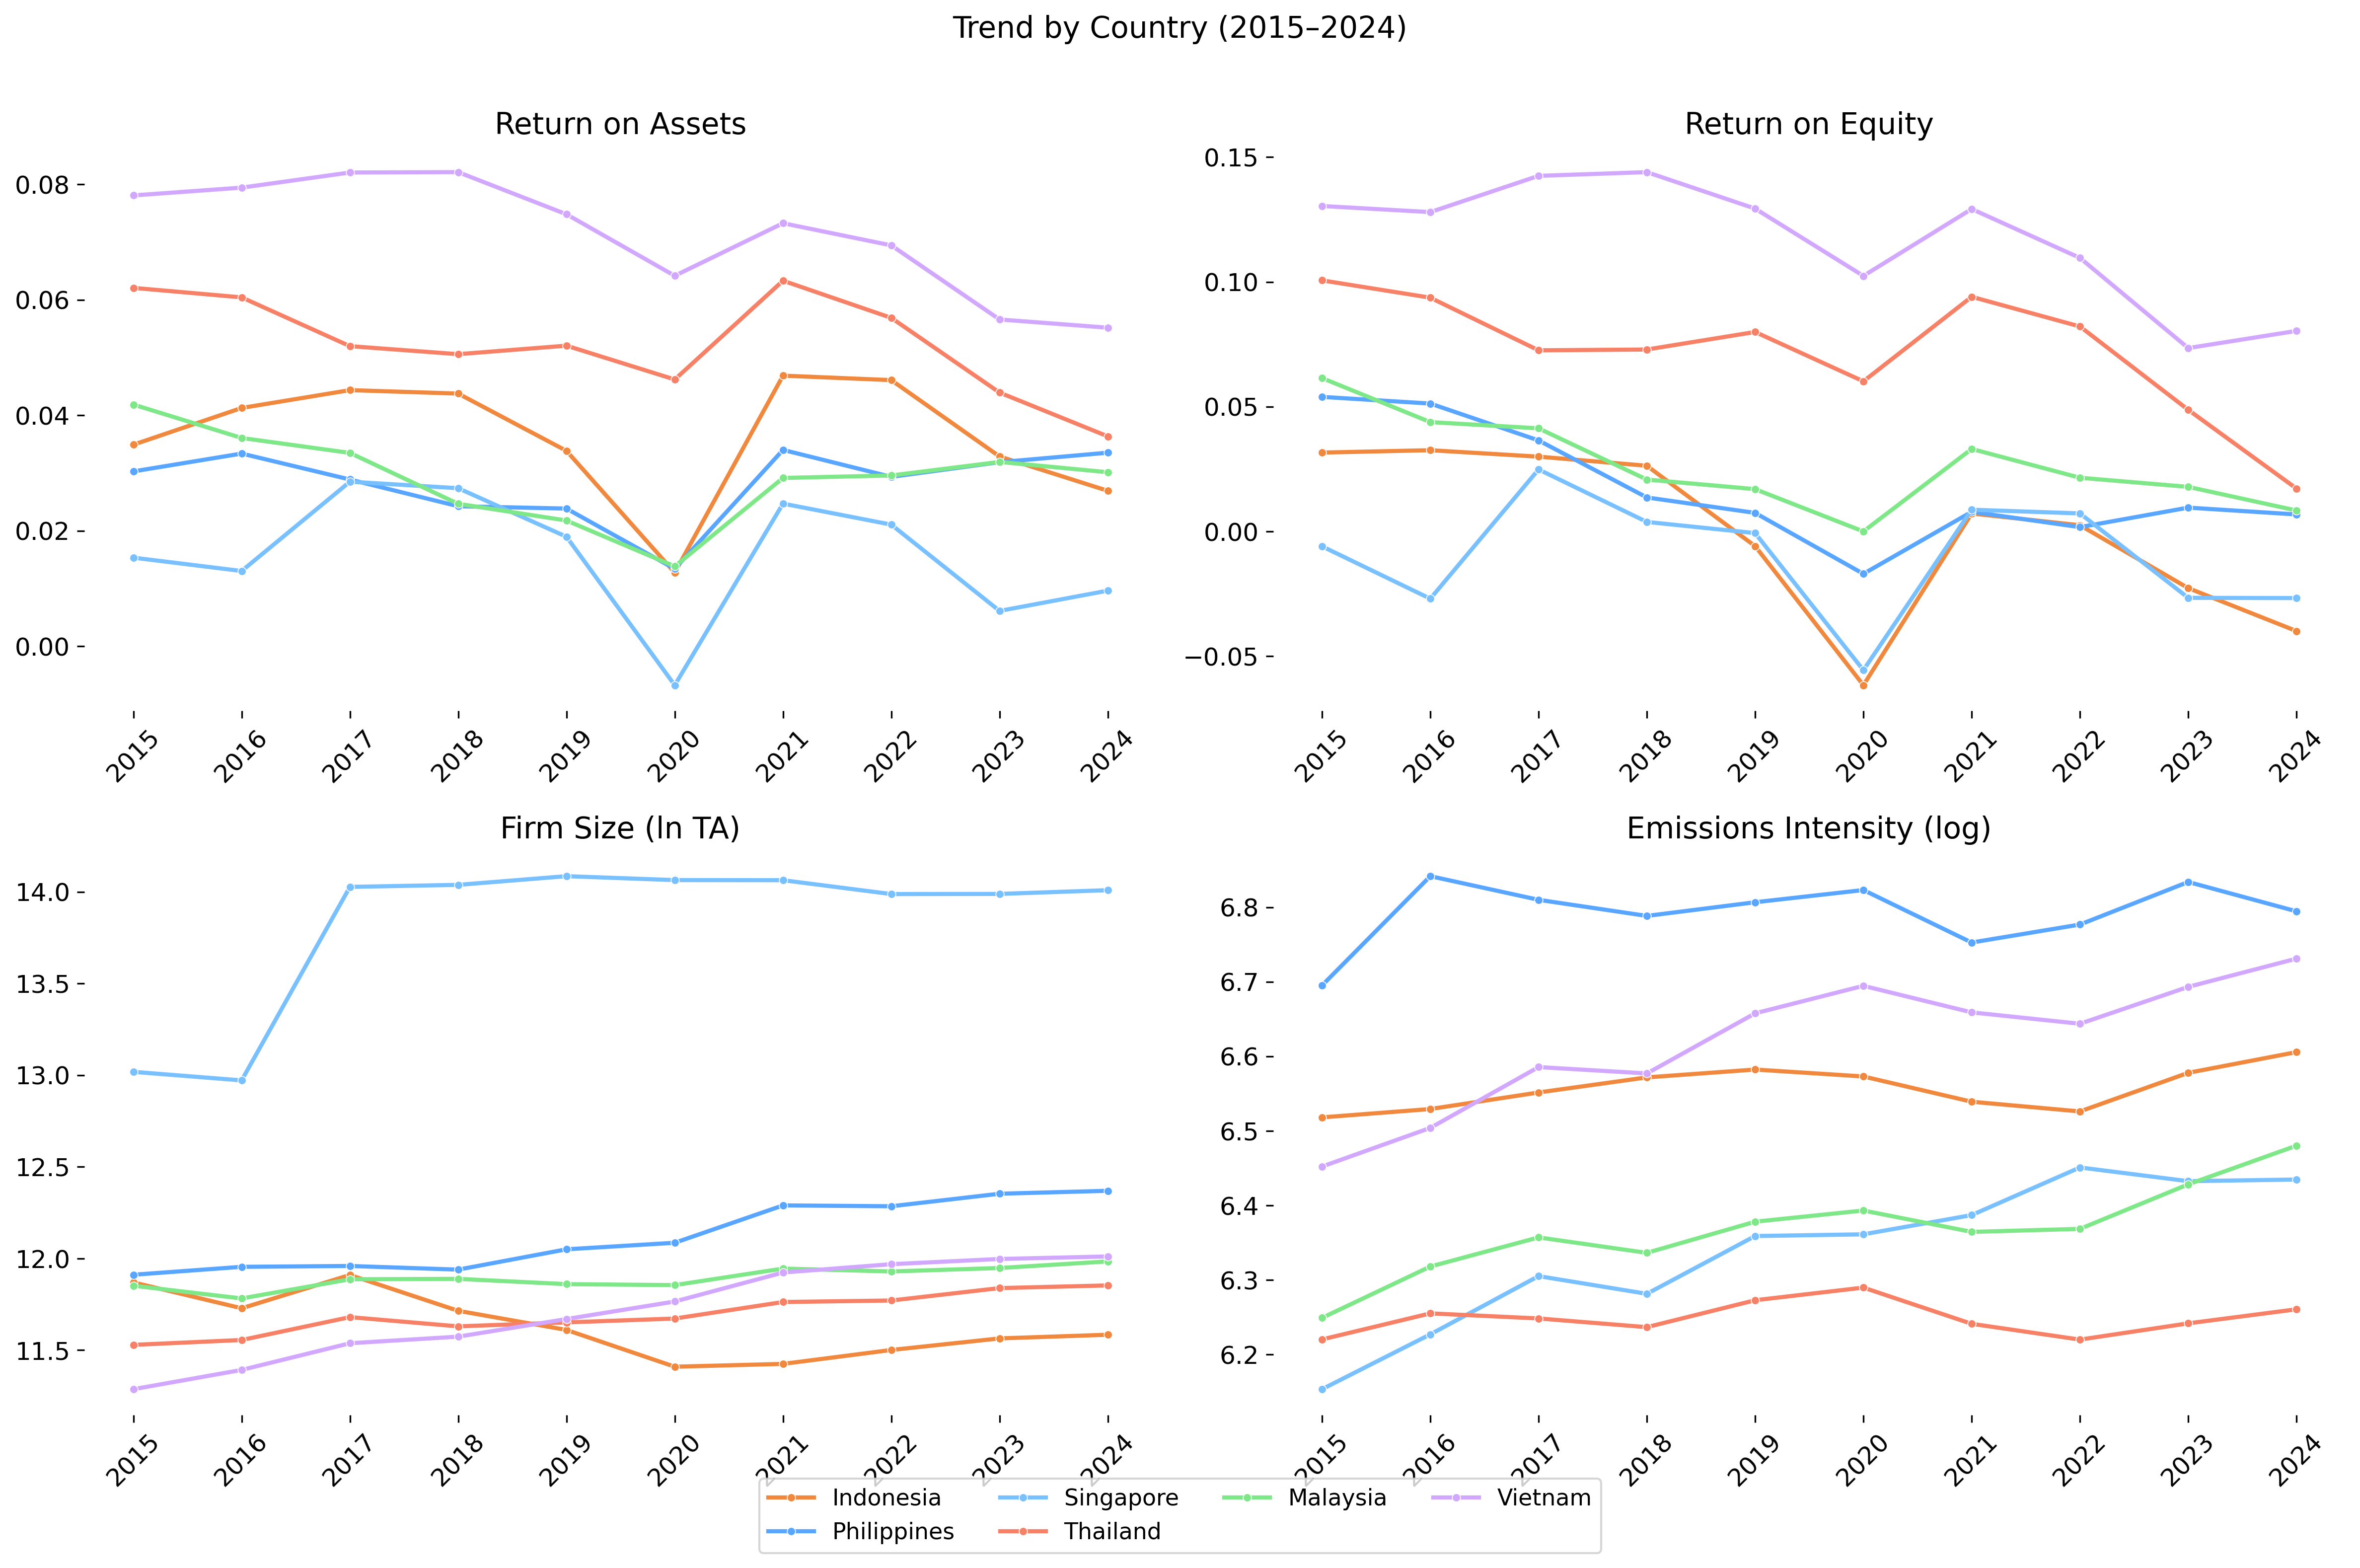
\includegraphics[width=0.95\textwidth]{../images/trend_analysis_country.png}
               \caption{\footnotesize Country-level trends for core financial and environmental variables.}
            \end{figure}
        \end{column}
        \begin{column}{0.35\textwidth}
            \small
            \textbf{Notes:}
            \begin{itemize}
                \item Disaggregates ASEAN-level averages from the main trend analysis.
                \item Reveals heterogeneous pandemic responses across markets.
                \item Supports country fixed effects in regression models.
            \end{itemize}
        \end{column}
    \end{columns}
\end{frame}

% Appendix B: Financial Health by Country
\begin{frame}{Appendix B: Financial Health by Country}
    \begin{columns}
        \begin{column}{0.65\textwidth}
            \begin{figure}
               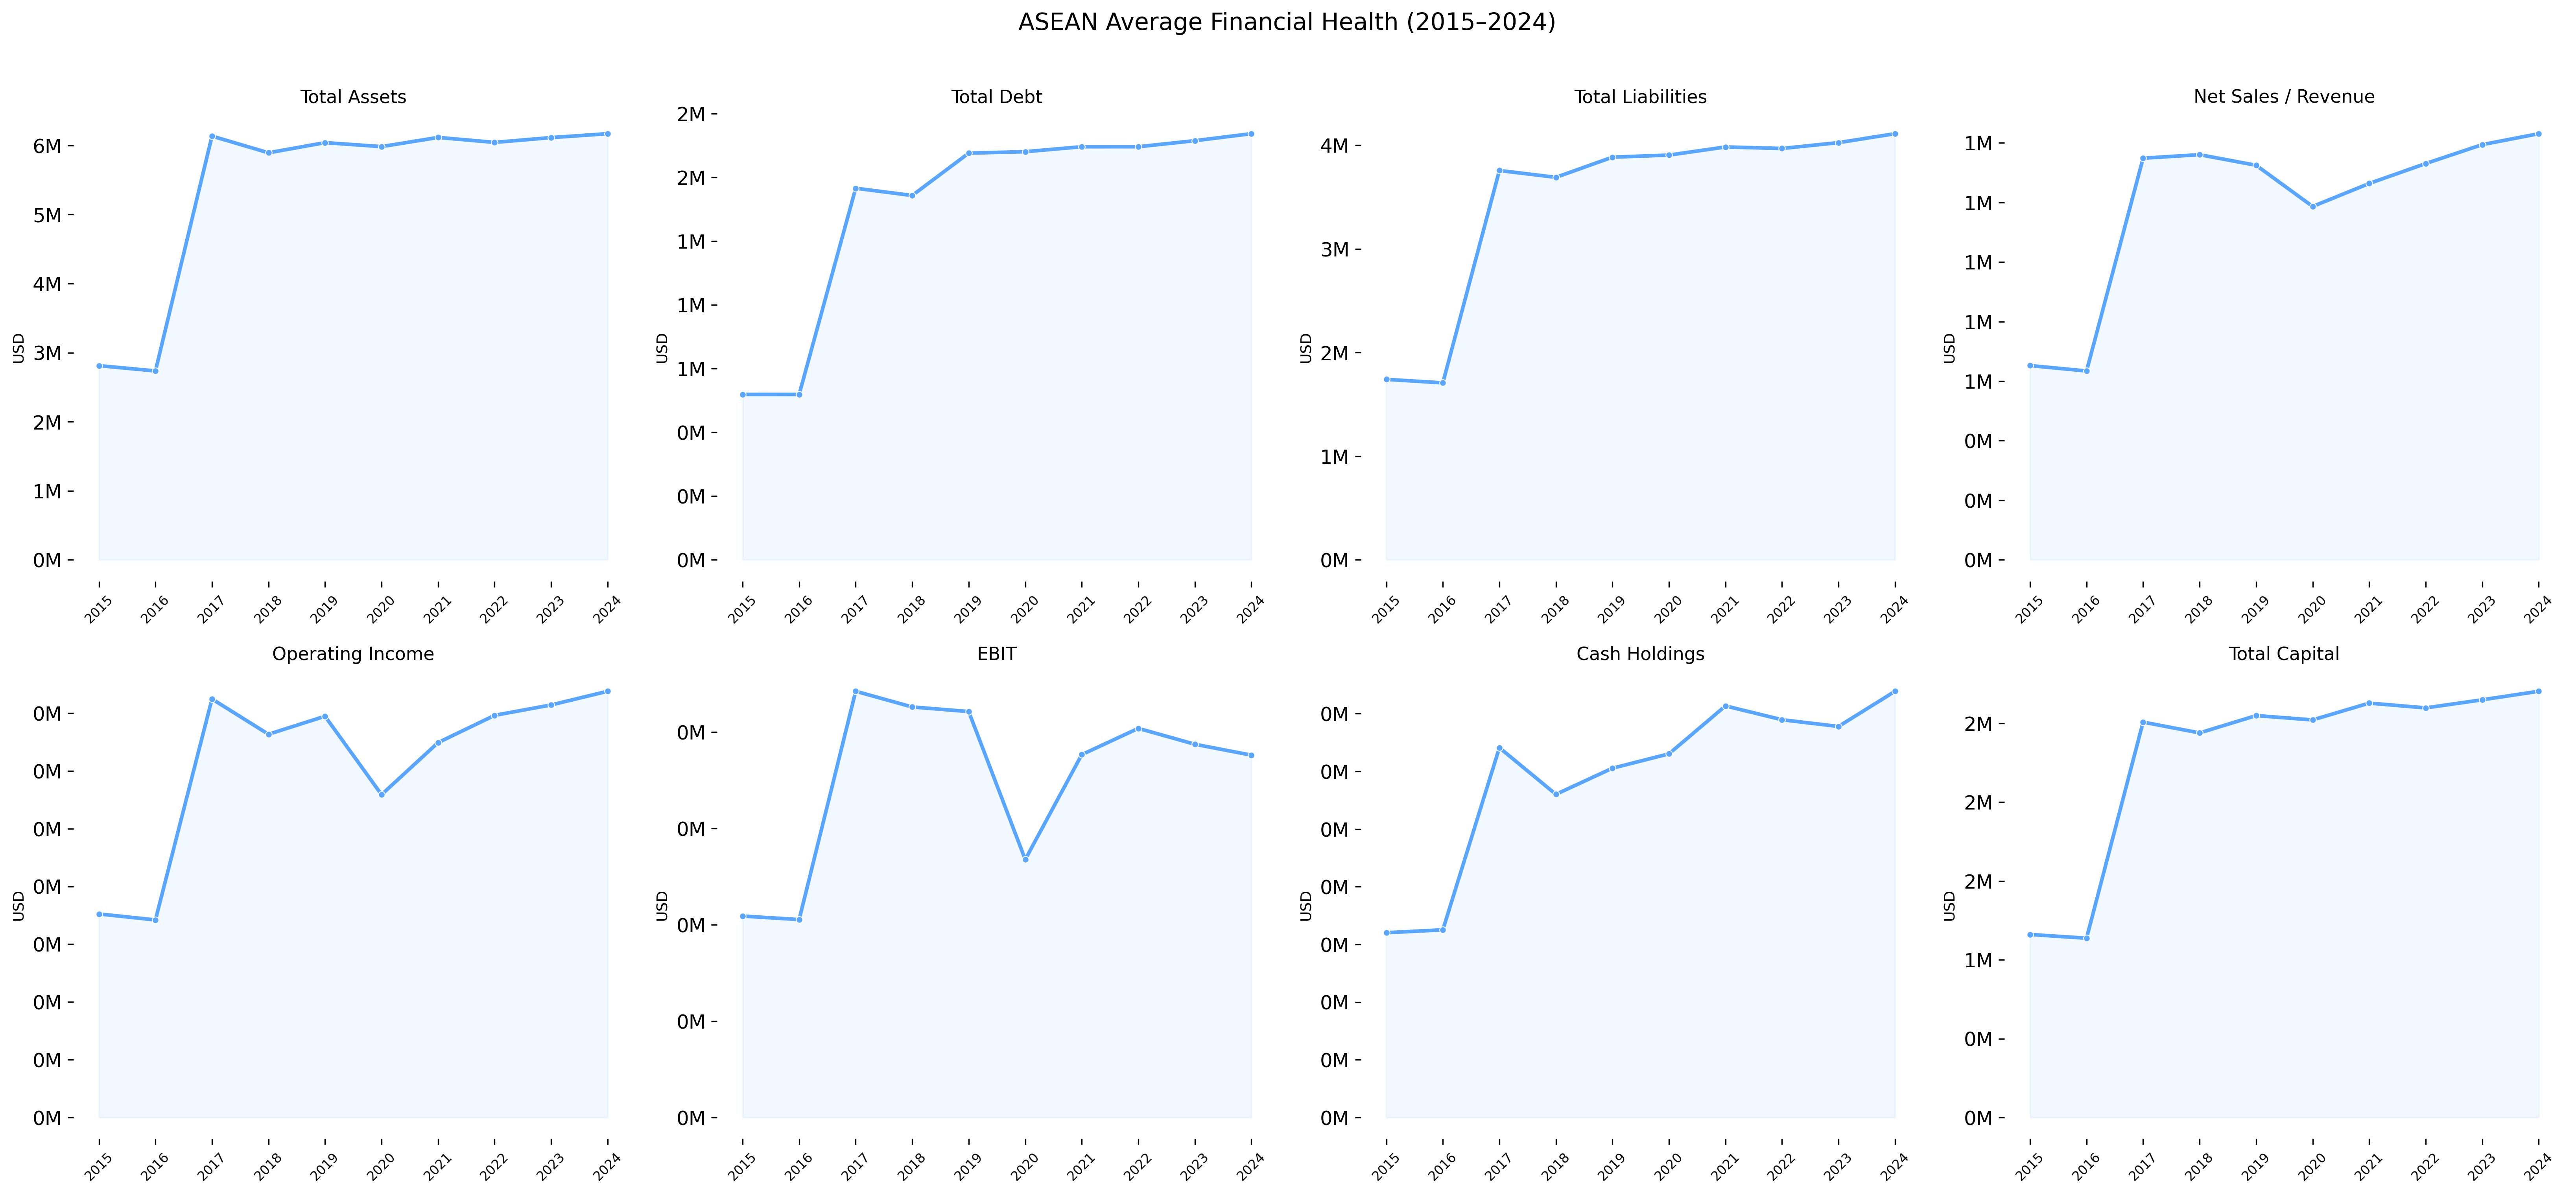
\includegraphics[width=\textwidth]{../images/financial_health.png}
               \caption{Total Assets, Revenue, Total Debt, and Operating Income by country.}
            \end{figure}
        \end{column}
        \begin{column}{0.35\textwidth}
            \small
            \textbf{Notes:}
            \begin{itemize}
                \item Singapore firms are significantly larger, compressing other countries on the scale.
                \item Operating Income drops sharply in 2020 across all countries.
                \item Total Debt shows a steady upward trend, particularly for Singapore.
            \end{itemize}
        \end{column}
    \end{columns}
\end{frame}

% Appendix C: Liquidity & Cash Flow Trends
\begin{frame}{Appendix C: Liquidity \& Cash Flow Trends}
    \begin{columns}
        \begin{column}{0.65\textwidth}
            \begin{figure}
               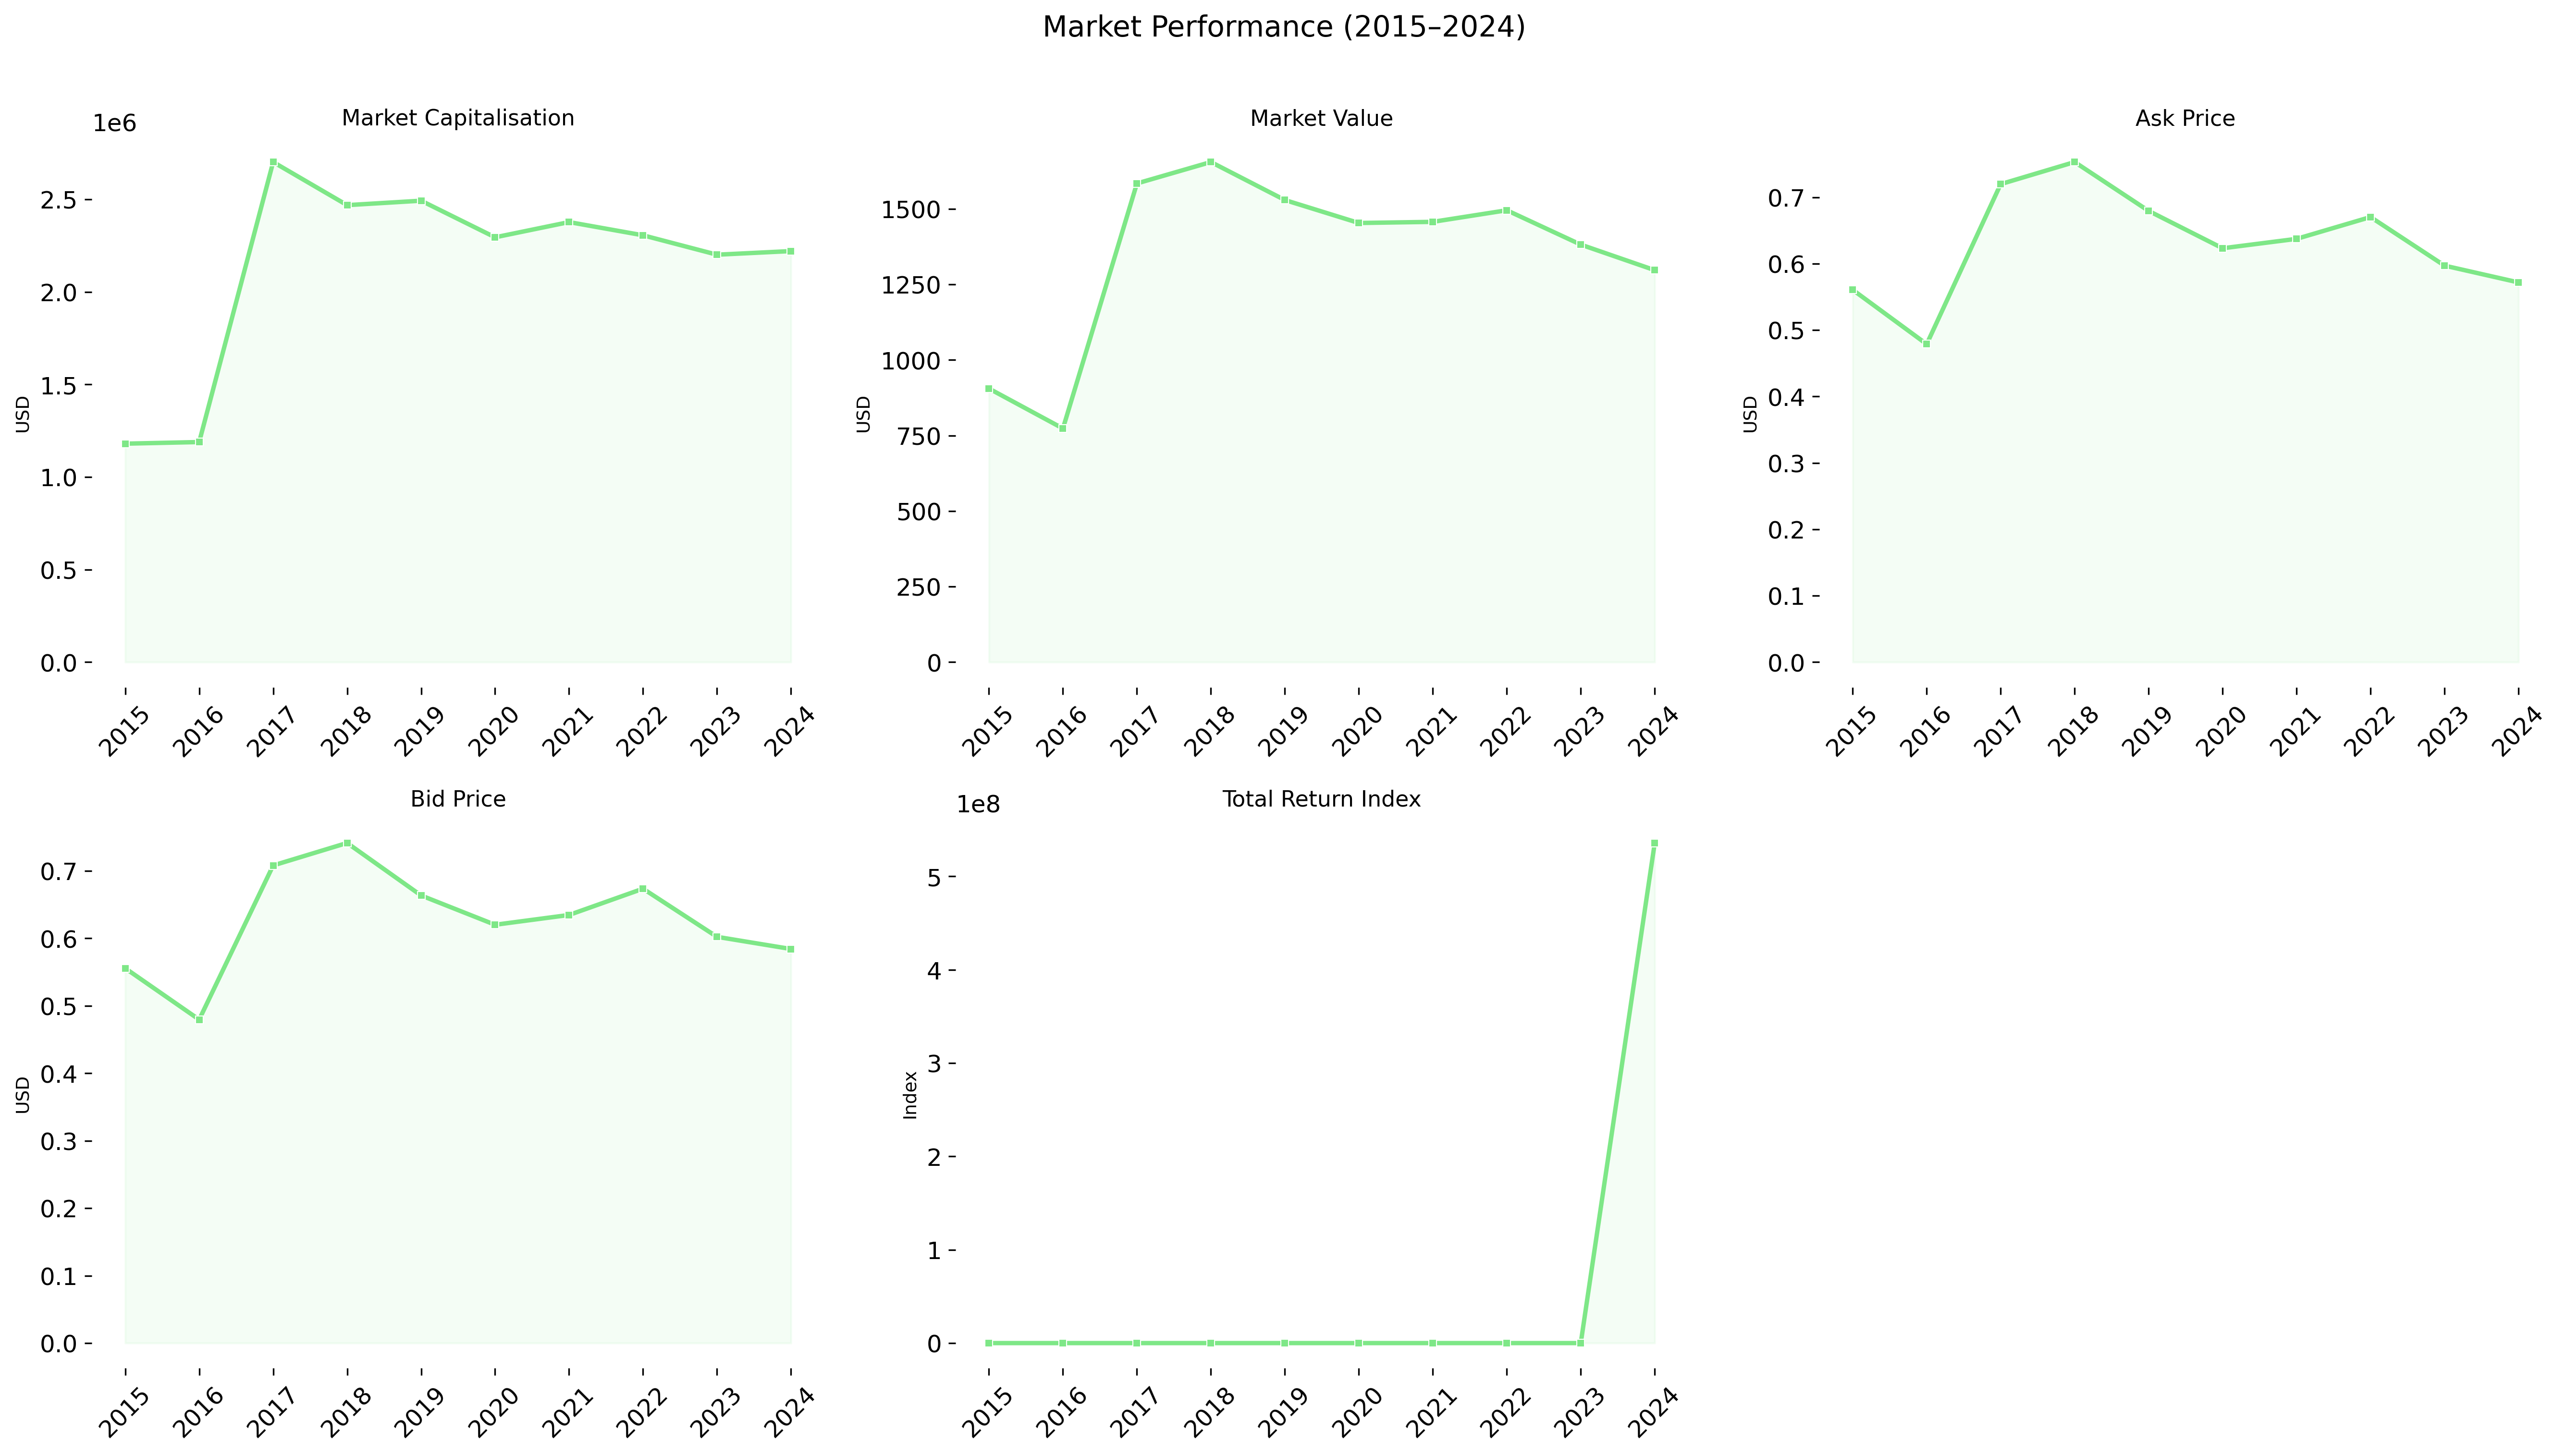
\includegraphics[width=\textwidth]{../images/liquidity_analysis.png}
               \caption{Panel-level liquidity and cash flow metrics (2015--2024).}
            \end{figure}
        \end{column}
        \begin{column}{0.35\textwidth}
            \small
            \textbf{Notes:}
            \begin{itemize}
                \item Working Capital dipped sharply in 2020 but recovered by 2021.
                \item Cash/Total Assets rose post-2020, stabilizing at a higher level---suggesting firms increased precautionary cash holdings.
                \item Supports the Cash-to-Assets $\times$ Green Bond interaction rationale.
            \end{itemize}
        \end{column}
    \end{columns}
\end{frame}

\end{document}
